\chapter{Signal Modelling}~\label{ch:SignalModelling}
\RaggedRight \parindent=25pt
In this chapter we discuss the MC generation of the ADD Large Extra Dimensions, Clockwork and the Unparticles - the three model interpretations used for our statistical analysis. 

\section{ADD Large ED Samples}~\label{subsec:MC_Signal_ADD}
The large extra dimensions model of Arkani-Hamed, Dimopoulos and Dvali
(ADD)~\cite{Arkani-Hamed:1998jmv, Arkani-Hamed:1998sfv} can produce diphoton events through virtual graviton exchange, leading to an enhancement of the diphoton invariant mass spectrum at large mass. Since the spacing between
Kaluza-Klein graviton states is typically small in the ADD scenario,
this effectively gives a continuum, non-resonant
enhancement.


We consider two conventions for the ADD signal, one having a positive interference with the Standard Model diphoton production process and another with negative interference. These conventions are equivalent to conventions by Giudice, Ratazzi and Wells (GRW) \cite{Giudice:1998ck}, and the one by Hewett \cite{Hewett:1998sn} which were explored in a previous paper~\cite{cmsdiphoton2016}. These are labeled as \texttt{NegInt-1} and \texttt{NegInt-0}, respectively \footnote{We found the convention choice in \PYTHIA a little odd for this parameter, so we note here that \PYTHIA default for the ADD model is to apply negative interference (paramater \texttt{NegInt} defaults to 0), and to turn this off, you have to set \texttt{NegInt=1}. This mislabeling was confirmed with Steve Mrenna. It results from the fact that the formula implemented within PYTHIA for the interference already has a minus sign built into it.}.

To span the entire mass spectrum, samples were produced in split mass bins from $\mgg = 500\GeV$ up to the value of $\Lambda_T$. Note that the ADD model is an effective theory that is only valid below $\Lambda_T$. The mass binning are split in such a way that a large effective luminosity is generated at higher masses so as to get better statistics. For illustration, the samples generated with $\Lambda_T = 9000$ have the following mass bins, 500--1000, 1000--2000, 2000--4000, 4000--9000.


The amplitude for a process involving virtual graviton exchange involves a sum over the Kaluza-Klein tower of graviton mass states.
This results in a higher dimension operator with coefficients suppressed by some mass scale~\cite{Gleisberg:2003ue}, which can be parametrized by $\eta_G = \mathcal{F}/M_S^4$, where $\mathcal{F}$ is a dimensionless parameter for which several conventions exist in the literature:

\begin{equation}
\label{eqn:add_f_conventions}
\mathcal{F} =
\begin{cases}
1 \quad \text{(GRW)}, \\
\log\left(\frac{M_S^2}{\hat{s}} \right) , \; \text{if} \; n_{ED} = 2 \\
\frac{2}{n_{ED} - 2} , \; \text{if} \; n_{ED} > 2 \\
\pm\frac{2}{\pi} \quad \text{(Hewett}),
\end{cases}
\text{(HLZ)} ,
\end{equation}
where $\sqrt{\hat{s}}$ is the center-of-mass energy of the colliding partons.
HLZ and GRW denote the names of the authors who introduced the convention: Han, Lykken and Zhang~\cite{Han:1998sg}; and Guidice, Rattazzi and Wells~\cite{Giudice:1998ck}.

The results of the 2016 nonresonant diphoton analysis were interpreted in each of these three scenarios. The results presented in this note use the GRW convention, with $\Lambda_{T} = M_{S}$, or the equivalent with negative interference, $\mathcal{F} = -1$ (as explained earlier, this change in convention is driven by the switch to ADD signal generation using PYTHIA, which uses a different ADD convention than the prior SHERPA usage in 2016).

The \mgg distributions for the signal samples are displayed in Figure~\ref{fig:ADDsignal} both before and after the subtraction of the SM background.
These plots were generated using the 2017 signal samples but the 2018 signal samples are similar.


% generated by Tools/bin/signal.cc
\begin{figure}[tbp!]
\begin{center}
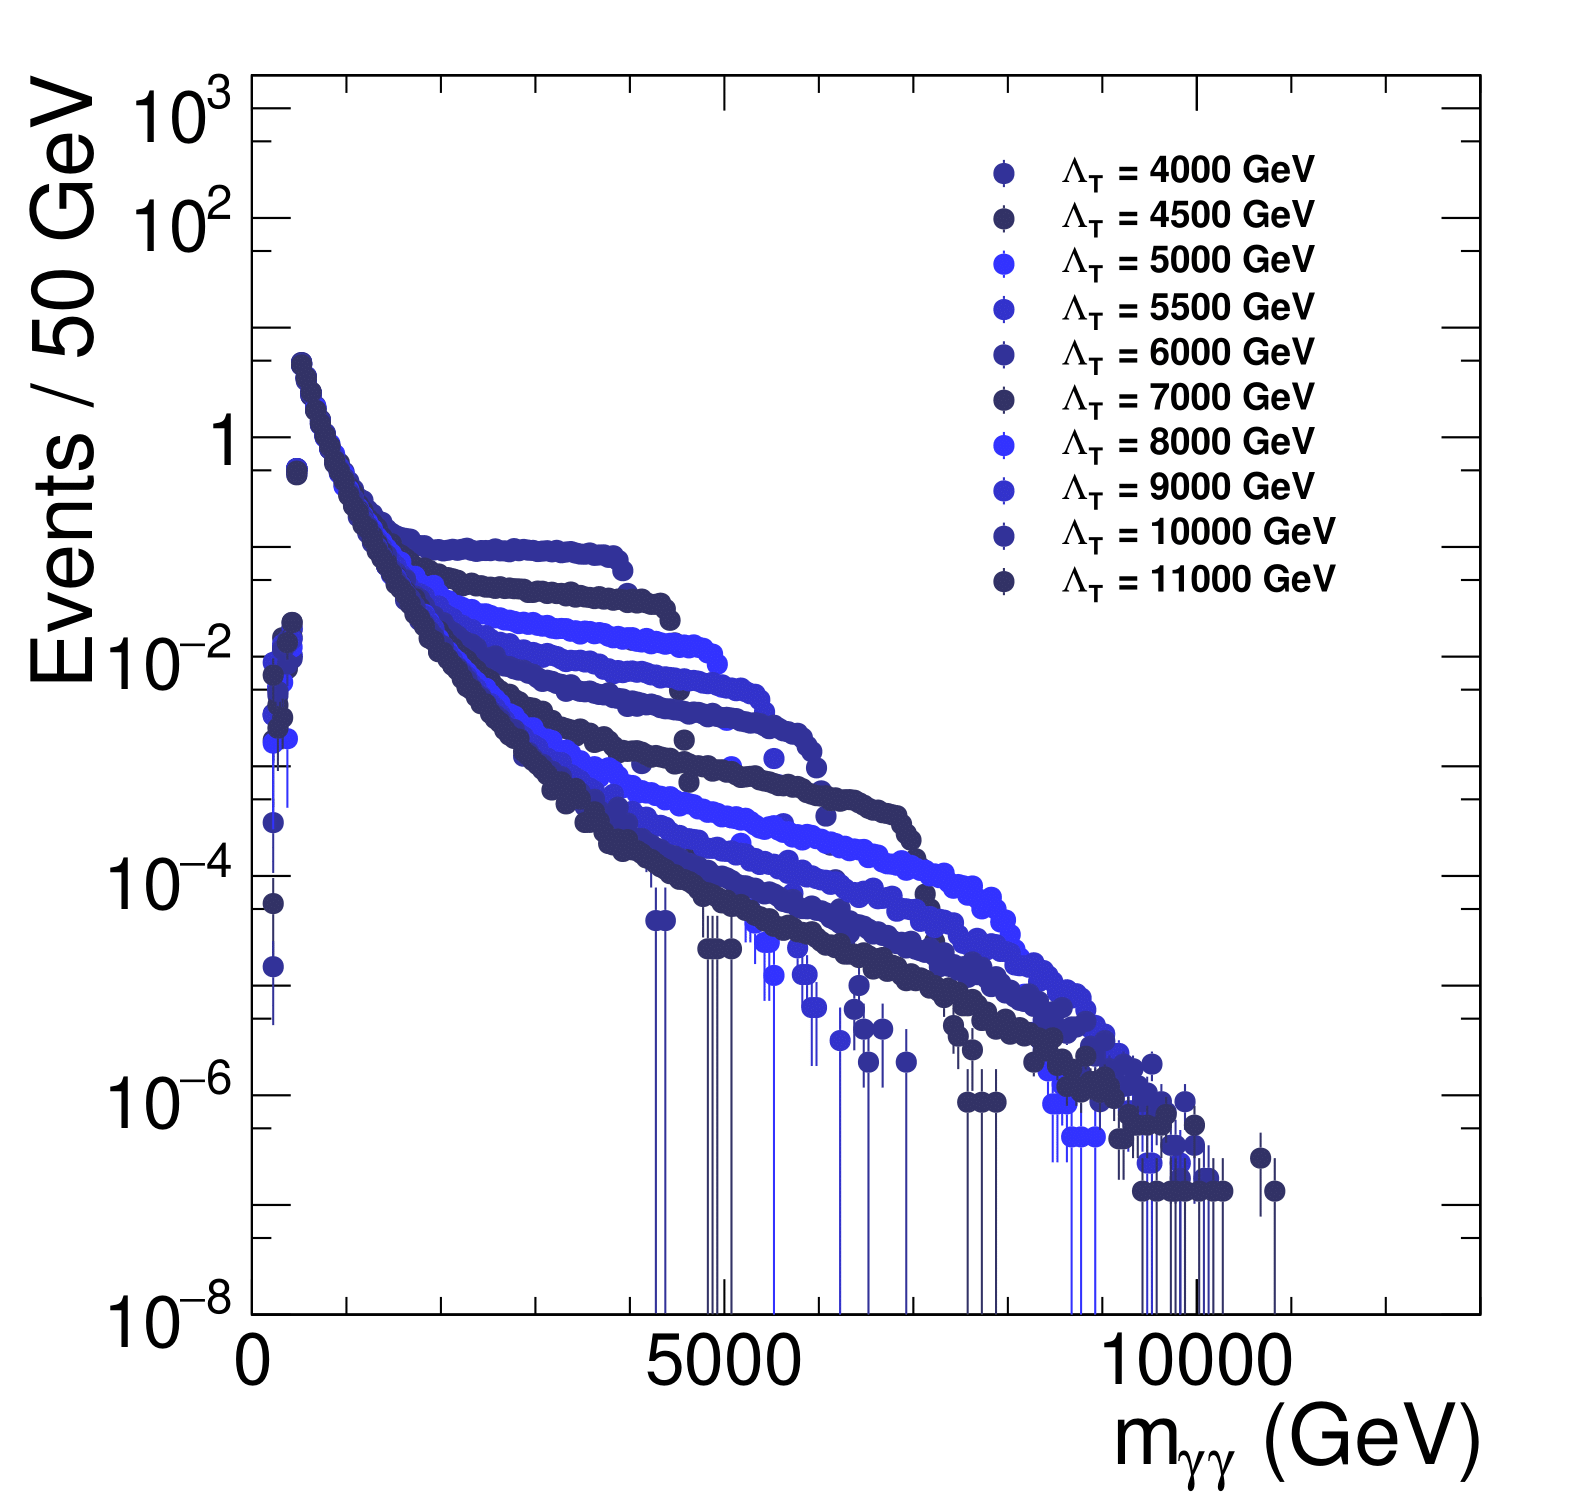
\includegraphics[angle=0,width=0.48\textwidth]{fig/ADDGravToGG_NED-2017_KK-1-1.png}
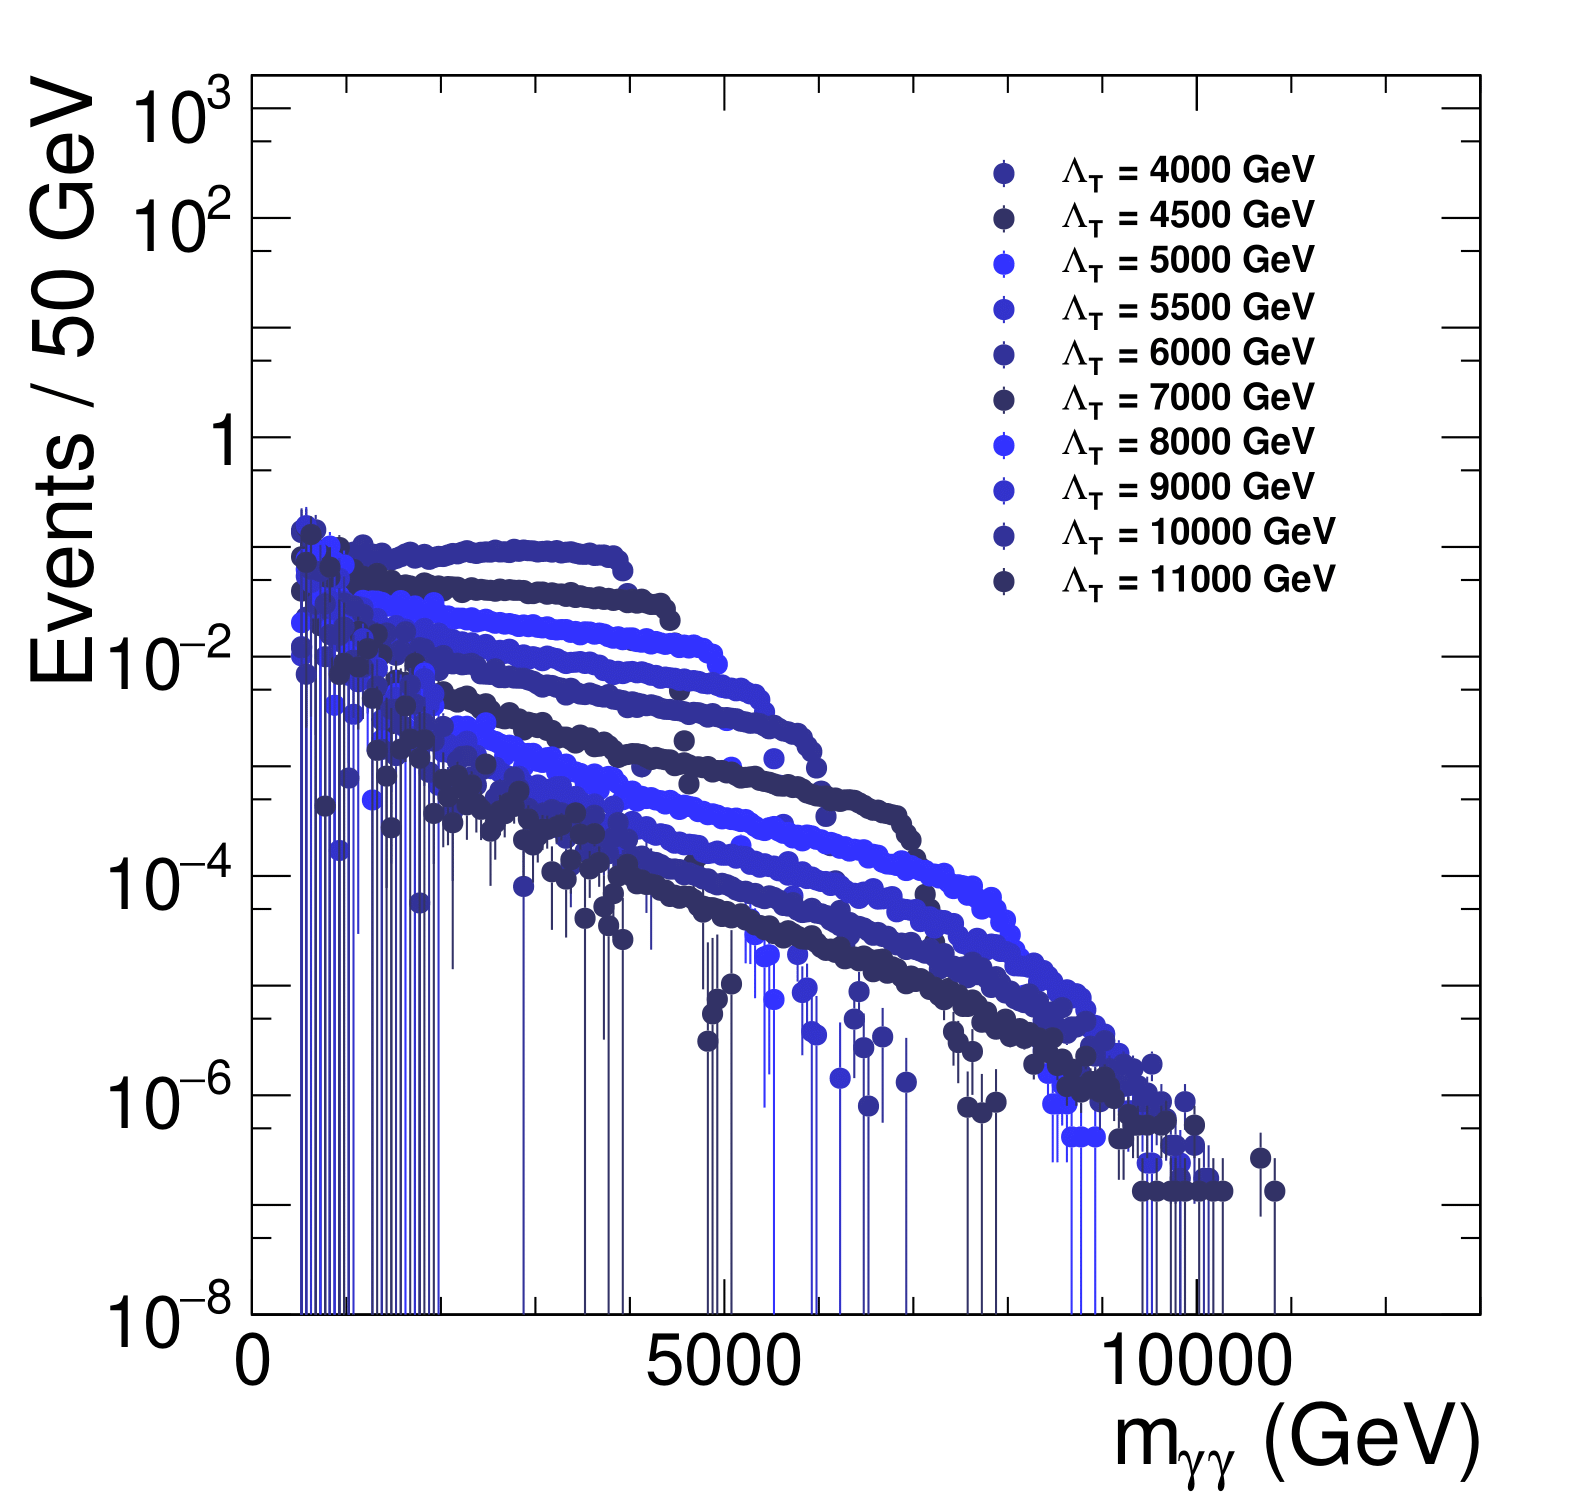
\includegraphics[angle=0,width=0.48\textwidth]{fig/ADDGravToGG_NED-2017_KK-1_bkg_sub-1.png}
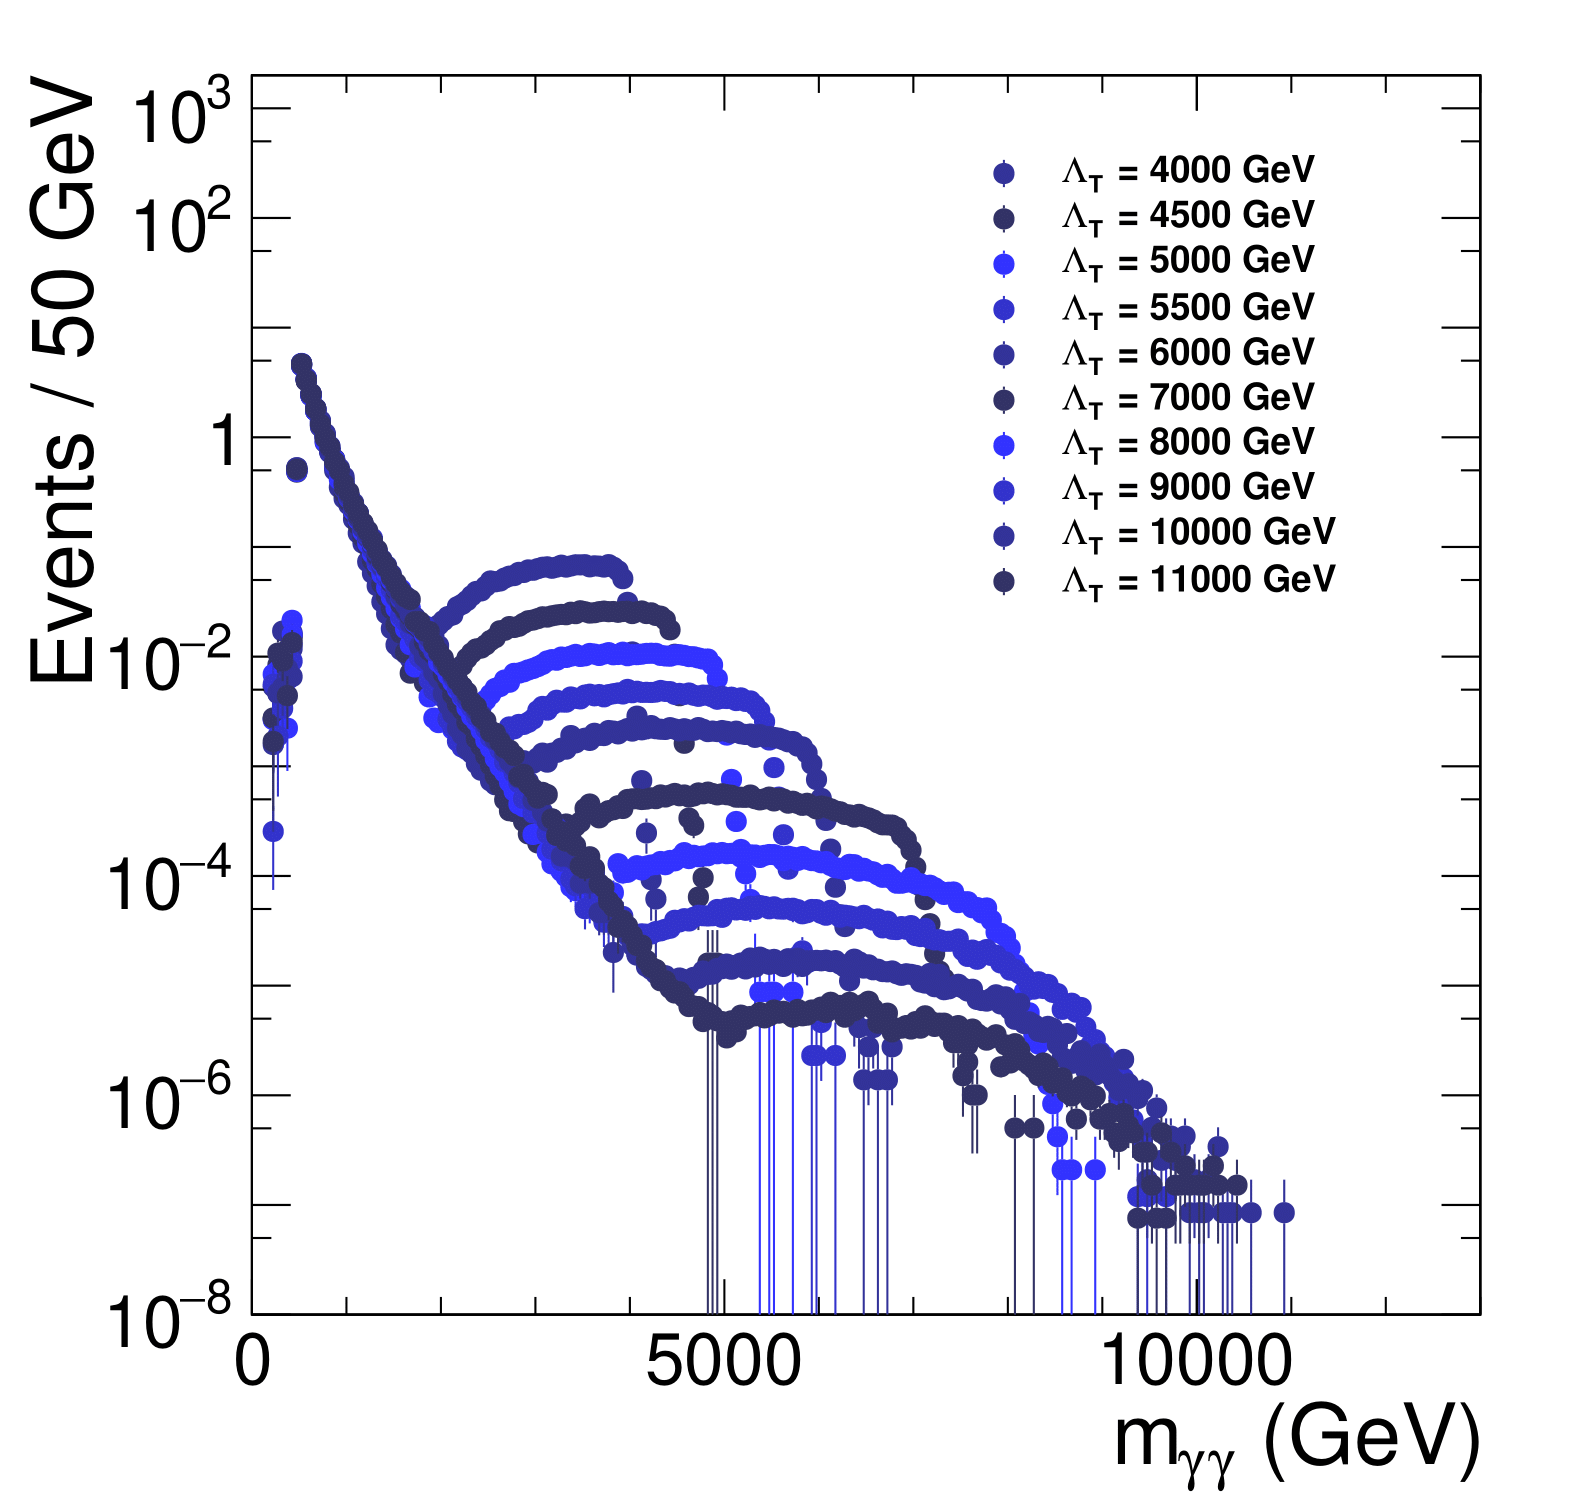
\includegraphics[angle=0,width=0.48\textwidth]{fig/ADDGravToGG_NED-2017_KK-0-1.png}
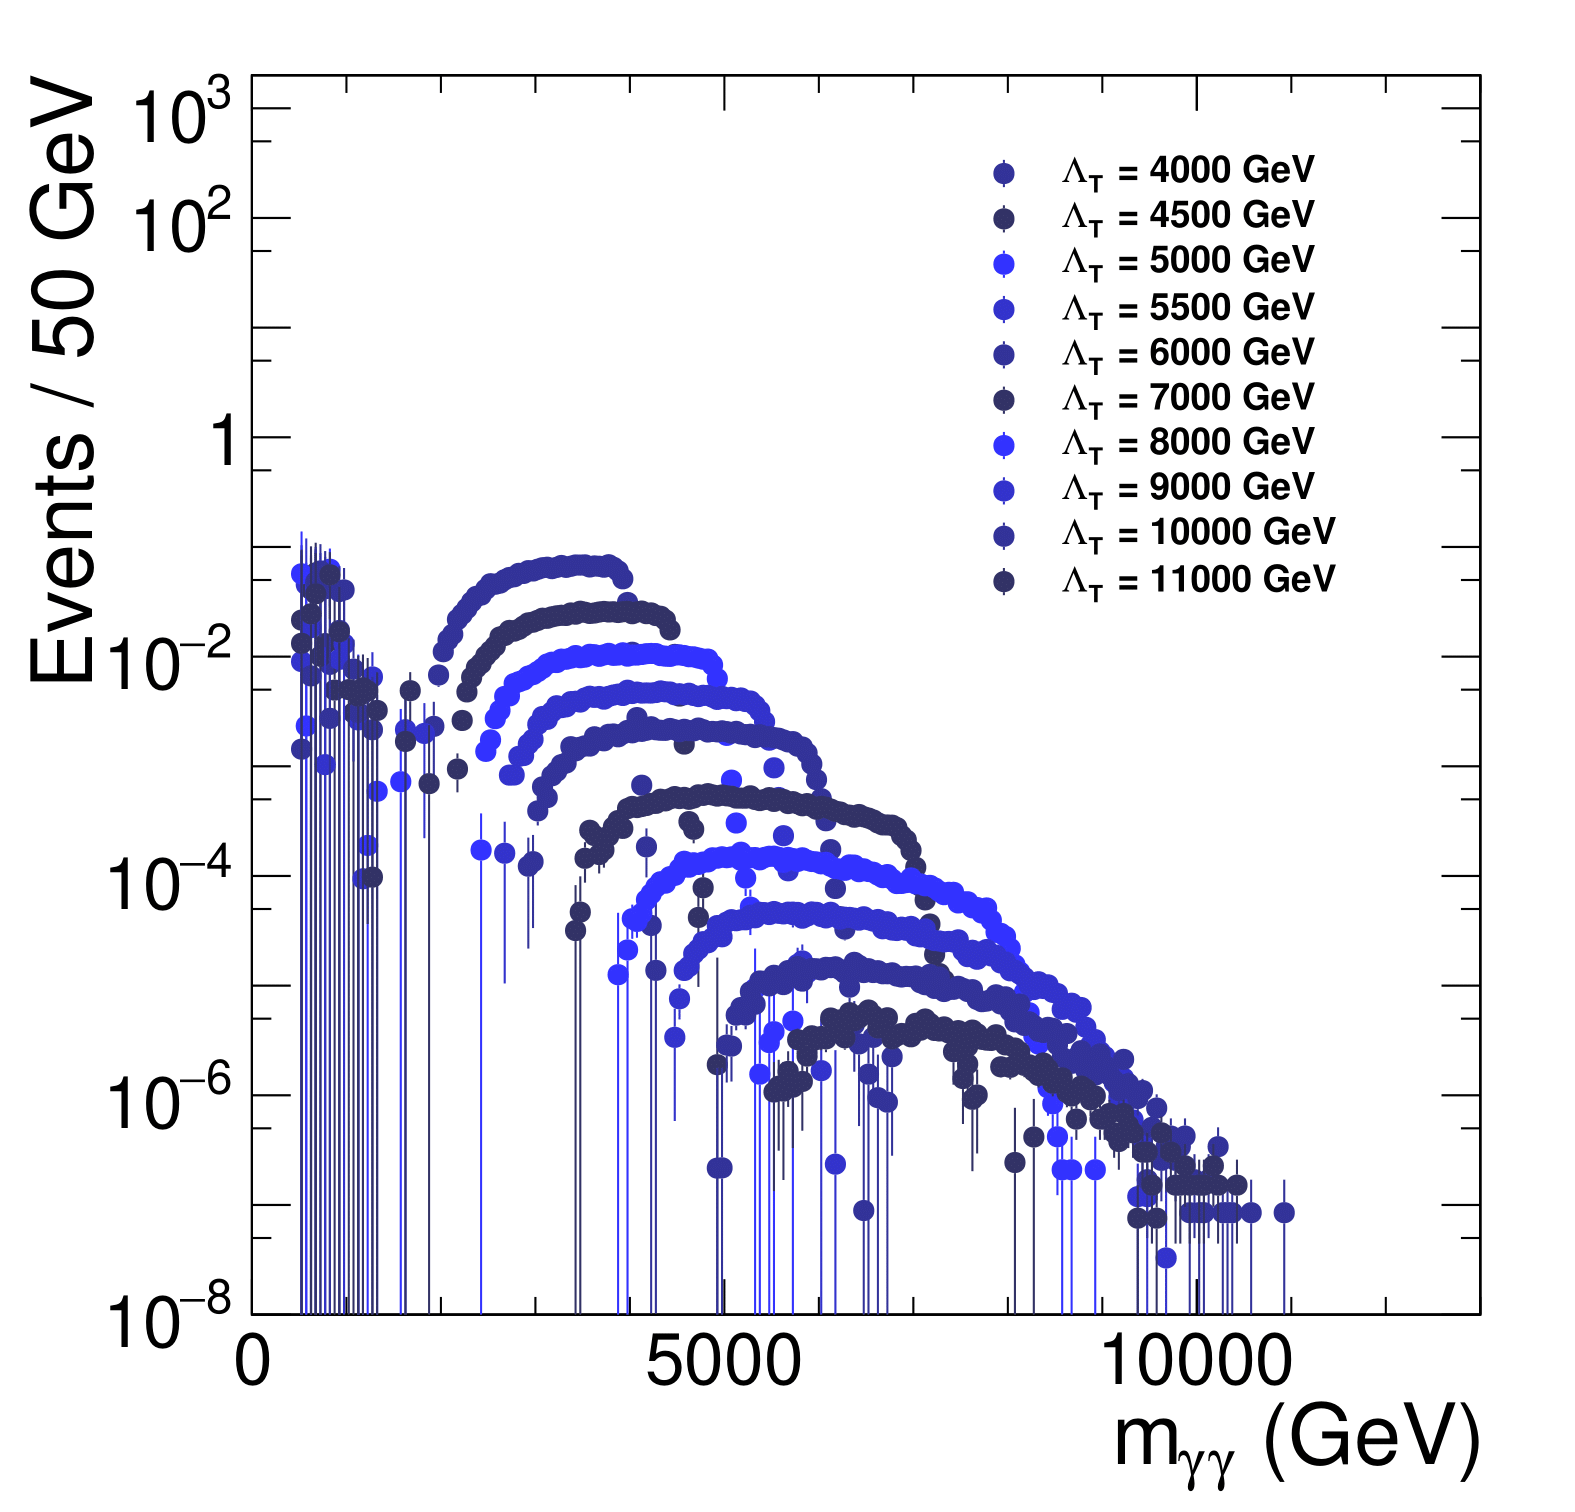
\includegraphics[angle=0,width=0.48\textwidth]{fig/ADDGravToGG_NED-2017_KK-0_bkg_sub-1.png}
\end{center}
\caption{The $m_{\gamma\gamma}$ distribution in signal events for the generated values of $\Lambda_T$ before (left) and after (right) subtraction of SM background. The upper(lower) plots show signals generated assuming positive (negative) interference with the SM background. The plots were generated using the 2017 ADD samples and are normaa
lized to an integrated luminosity of 1\fbinv.
}
\label{fig:ADDsignal}
\end{figure}

The ADD signal samples (Table~\ref{table:ADDsamples}) used for the analysis were produced at leading order (LO) using \PYTHIA~8.2~\cite{Sjostrand:2008za} with the \texttt{NNPDF}~3.1 LO set of parton distribution functions included in the underlying event tune, \texttt{TuneCP2}. In the context of Pythia, ``Tunes" refers to specific sets of parameters used to configure the event generator for simulating particle collision events. Previously, for our 2016 analysis~\cite{Sirunyan:2018wnk} , the samples were generated with a built-in implementation of the ADD model in \SHERPA~2.1.1;  but later \SHERPA versions moved to using Universal FeynRules Output (UFO) interface~\cite{Degrande:2011ua} and removed the built-in ADD implementation. The UFO interface makes use of the FeynRules package in Mathematica, which assists in the generation of Feynman diagrams for specific particle physics models. The output is then saved to a format that can be used as an input to Monte Carlo generators such as \SHERPA to generate events associated with the physics models. The Large Extra Dimensions (LED) implementation with the UFO presented some difficulties in interfacing with \SHERPA, so we switched to using \PYTHIA~8 which already has the ADD model built-in. Other related analyses, for example the dilepton~\cite{CMS:2021ctt, Sirunyan:2019} and dijet channels~\cite{CMS:2017caz} have also used \PYTHIA~8. In \PYTHIA~8, the ADD model is parametrized by the $\Lambda_T$ variable which is the ultraviolet cutoff parameter for the virtual graviton exchange process.

% The term "TuneCP2" in the context of Pythia refers to a specific set of parameters used to configure the Pythia event generator for simulating particle collisions in high-energy physics experiments. Pythia is a widely used software package for simulating the production and decay of high-energy particles in various collider experiments.

% "Tuning" in this context refers to the adjustment of the model parameters within Pythia to better match experimental data. The CP2 part of the name likely indicates that it is part of the CTEQ-TEA (Coordinated Theoretical-Experimental Project on QCD Theory and Experiment Analysis) package, which provides parton distribution functions (PDFs) for use in high-energy physics calculations.

As the ADD signal results in the same final state as the SM
background, interference effects are large in the regions of phase space where the signal and background amplitudes are comparable.
To take this effect into account, the signal samples are generated including both the signal and SM background amplitudes.
Additional samples generated identically, but excluding the signal contribution, are used to subtract the SM background, leaving the contributions of
signal and the interference between signal and background. These samples are listed in a table in the previous section.

It is not computationally feasible to include additional partons in
the matrix element in the signal plus background samples, and so
additional partons are not included in the either the 
signal+background or background-only samples.

Though the \textrm{GG} samples used to subtract the background from the ADD signal (which includes the SM interference and background) are generated with \PYTHIA~8 while the \textrm{GGJets}
samples are generated with \SHERPA, it is not necessary to use the same generator; the background prediction is not used in constructing the signal distributions and vice versa, so there is
no need for consistency. The only other difference between these background samples and those used in the background prediction is an increase of the photon \pt requirement at
generator level from 50\GeV to 70\GeV, which does not affect the
analysis since the actual \pt threshold used in the analysis exceeds both.

These background samples include a small contribution from the gluon-gluon-initiated box diagram.
This box diagram is not included in the simulation of the ADD signal and so, in order to avoid over-subtracting the background, we exclude events from the $\gamma\gamma$ background subtraction samples that have PDG ID equal to 21. Figure~\ref{fig:ADDsignal_and_GG} demonstrates, in the low \mgg region, for a signal sample with negligible signal contribution in this region, the agreement between the ADD signal and quark-antiquark background alone. 

% The GG background subtraction samples include an additional gluon-gluon-initiated box diagram that is not present in the ADD signal+interference+background samples. This extra component is excluded at analysis level.

% generated by Tools/bin/gg_bkg_sub.cc
\begin{figure}[htbp!]
\caption{A representative ADD sample signal agreement with the quark-antiquark background (light blue) alone in the low \mgg region.}
\begin{center}
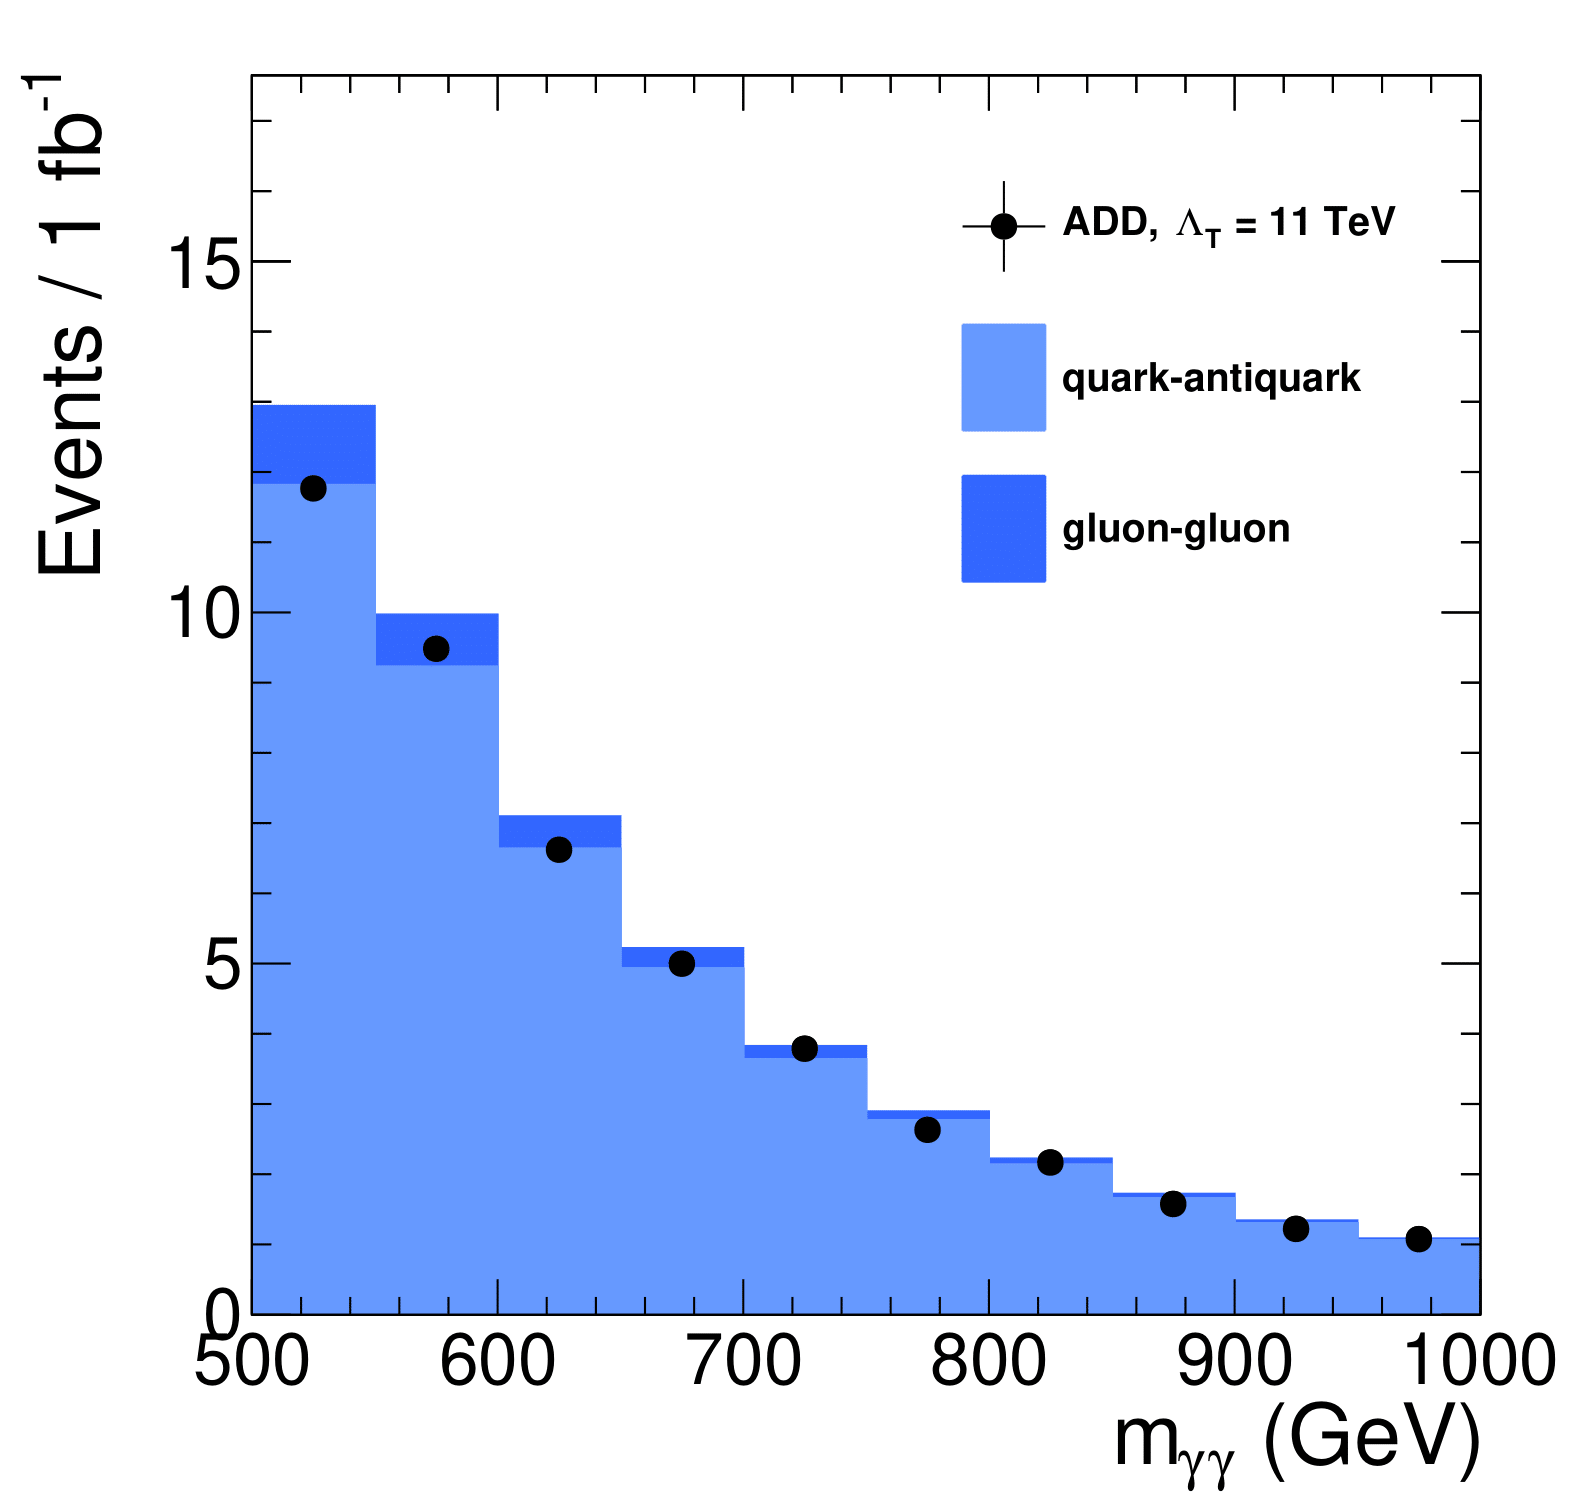
\includegraphics[angle=0,width=0.48\textwidth]{fig/GG_bkg_sub-1.png}
\end{center}
\label{fig:ADDsignal_and_GG}
\end{figure}




\subsection{Clockwork Model}

% Models with extra-dimensions are attempts to address the Hierarchy Problem in the Standard Model of Particle Physics.
% One such model is called the Continuum Clockwork Mechanism~\cite{2Clockwork} which coincides with a five-dimensional gravitational theory on a linear dilaton background~\cite{3LittleStringTheoryAtATeV, 4LittleStringTheoryAtATeV}.
% The clockwork mechanism is a general mechanism that can take large effective interaction scales from dynamics occuring at much lower energies.
% This is achieved by introducing N copies of some particle content on different sites forming a one-dimensional lattice in theory space.
% The physical mass spectrum results in a single massless mode localised on the end site of the lattice and a set of massive modes ('gears') distributed along the sites.
% In the continuum limit of the clockwork with $N\rightarrow \infty$, this lattice is interpreted as a physical extra dimension and the gears play the role of the KK modes.
% It has been shown~\cite{2Clockwork} that, in this limit, the clockwork theory corresponds to the linear dilaton theory, which can be independently motivated by dual constructions of Little String Theory~\cite{3LittleStringTheoryAtATeV}.
% The usual massless graviton is accompanies by an infinite tower of massive spin-2 graviton gears with a characteristic pattern of masses and couplings. In particular, the masses of the graviton gears can be so densely distributed, as in the KK-modes of the Large Extra Dimensions, to produce an approximately continuous contribution to the diphoton spectrum as a function of $m_{\gamma\gamma}$~\cite{8GiudiceWIP}.

To generate the Clockwork signal, we make use of the ADD Large Extra Dimensions samples and translated them to produce the Clockwork Prediction. In the Clockwork model, the KK modes are all on shell, so there is no interference effect. The direct term for the ADD expression for the total cross section can be rescaled by

\begin{equation}
\theta(m_{\gamma\gamma} - k ) \frac{30 \Lambda^{8}_{T}}{283 \pi M_{5}^{3} } \sqrt{1-\frac{k^2}{m^{2}_{\gamma\gamma}}} \frac{1}{m^5_{\gamma\gamma}} \left[ 1+ \frac{5^2\cdot 7 \cdot 17}{283\cdot 2^8} \left(1-\frac{k}{m_{\gamma\gamma}}\right)^9 \sqrt{\frac{m_{\gamma\gamma}}{k}} \right]
\label{eq:rescalingfactorCW}
\end{equation}

where $\Lambda_{T}$ is equivalent to $M_{s}$ in the GRW convention, $M_{5}$ is the fundamental scale of the gravitational interactions analogous to the fundamental Planck scale $M_{D}$ in the ADD model, and $k$ is called the clockwork spring. The clockwork spring sets the inverse size of the extra dimension. Phenomenologically, it also controls the energy scale at which the KK modes can be excited. Perturbativity constrains $k <M_{5}$. The direct term for the ADD expression is the third term in the equation for the total cross section for the SM plus the ADD:

\begin{equation}
\sigma_{total} = \sigma_{SM} + \frac{\mathcal{F}}{M^4_{S}} \sigma_{int}+\frac{\mathcal{F}}{M^8_{S}} \sigma_{ADD} 
\label{eq:totalADDxsec}
\end{equation}

where $\mathcal{F}$ is defined in Eq.~\ref{eqn:add_f_conventions}.

% \begin{equation}
% \mathcal{F}=
%     \begin{cases}
%         1 & \text{if } \textit{GRW} \\
%         log\left(\frac{M^2_s}{\hat{s}}\right) & \text{if } n_{ED} = 2 \\
%         \frac{2}{n_{ED} - 2} & \text{if } n_{ED} > 2 \\
%         \pm \frac{2}{\pi} & \text{if } \textit{Hewett}
%     \end{cases}
%     \label{eq:KKConventions}
% \end{equation} 

% \begin{equation}
% \mathcal{F}=
%     \begin{cases}
%         1 & \text{if } x \in \mathbb{Q}\\
%         log\left(\frac{M^2_s}{\hat{s}}\right) & \text{if } x \in \mathbb{R}\setminus\mathbb{Q}
%     \end{cases}
% \end{equation}

% Here $\hat{s}$ is the centre-of-mass energy of the colliding partons.

% The different ADD conventions were generated with Pythia8. \FIXME{Write more on how the ADD samples were generated for the thesis}. 

We can take the linear combination of the SM-background subtracted positive interference GRW and the negative interference Hewett samples, given by the equations:

\begin{equation}
\sigma_{GRW} = \frac{1}{M^4_{s}} \sigma_{int} + \frac{1}{M^8_{s}} \sigma_{ADD}
\label{eq:GRWMs}
\end{equation}

\begin{equation}
\sigma_{Hewett} = \frac{-2/\pi}{M^4_{s}} \sigma_{int} + \frac{4/\pi}{M^8_{s}} \sigma_{ADD}
\label{eq:HewettMs}
\end{equation}

We can use Eq.~\ref{eq:KKConventions} to simplify and rewrite Eqs.~\ref{eq:GRWMs} and \ref{eq:HewettMs} in terms of $\Lambda_{T}$:

\begin{equation}
\sigma_{GRW} = \frac{1}{\Lambda^4_{T}} \sigma_{int} + \frac{1}{\Lambda^8_{T}} \sigma_{ADD}
\label{eq:GRWLambdaT}
\end{equation}

\begin{equation}
\sigma_{Hewett} = \frac{-1}{\Lambda^4_{T}} \sigma_{int} + \frac{1}{\Lambda^8_{T}} \sigma_{ADD}
\label{eq:HewettLambdaT}
\end{equation}

Combining these two we get the direct term:

\begin{equation}
\sigma_{ADD} = \frac{\sigma_{GRW}+\sigma_{Hewett_{-}}}{2}
\label{eq:GRWLambdaT}
\end{equation}

It is this equation that is rescaled by Eq.~\ref{eq:rescalingfactorCW} to produce the clockwork spectrum. We are careful to use the generator-level value of $M_{\gamma\gamma}$ rather than the reconstructed $m_{\gamma\gamma}$ to do the rescaling.

% \begin{figure}[htbp!]
%     \centering
%     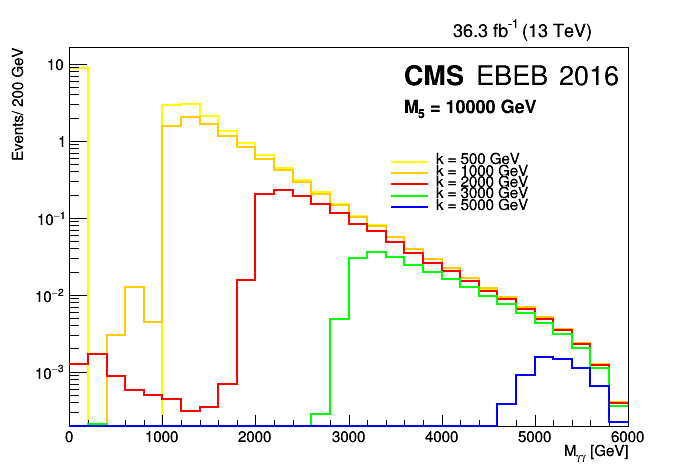
\includegraphics[angle=0,width=0.48\textwidth]{fig/2016EBEB.png}\hspace{0.04\textwidth}
%     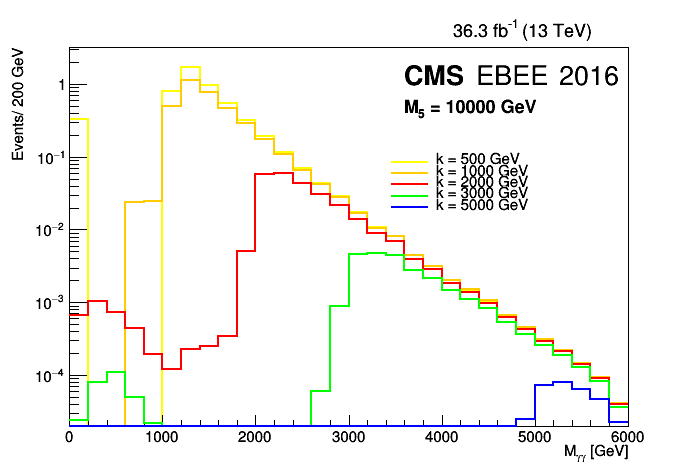
\includegraphics[angle=0,width=0.48\textwidth]{fig/2016EBEE.png}\\[0.5em]
%     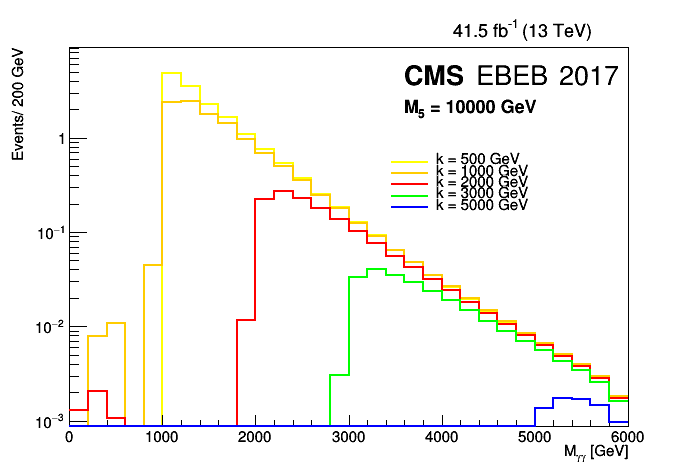
\includegraphics[angle=0,width=0.48\textwidth]{fig/2017EBEB.png}\hspace{0.04\textwidth}
%     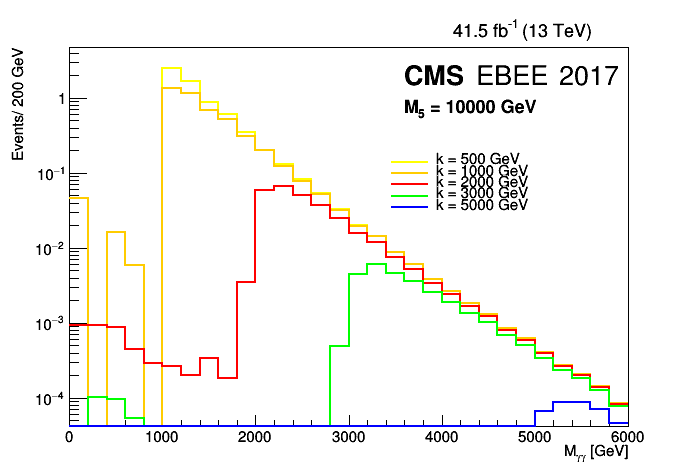
\includegraphics[angle=0,width=0.48\textwidth]{fig/2017EBEE.png}\\[0.5em]
%     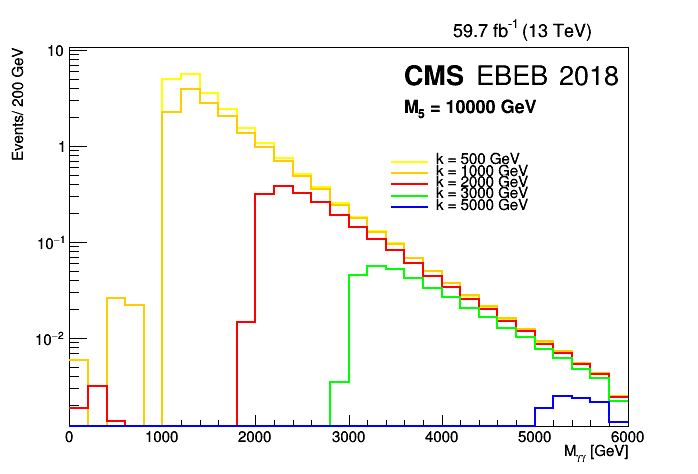
\includegraphics[angle=0,width=0.48\textwidth]{fig/2018EBEB.png}\hspace{0.04\textwidth}
%     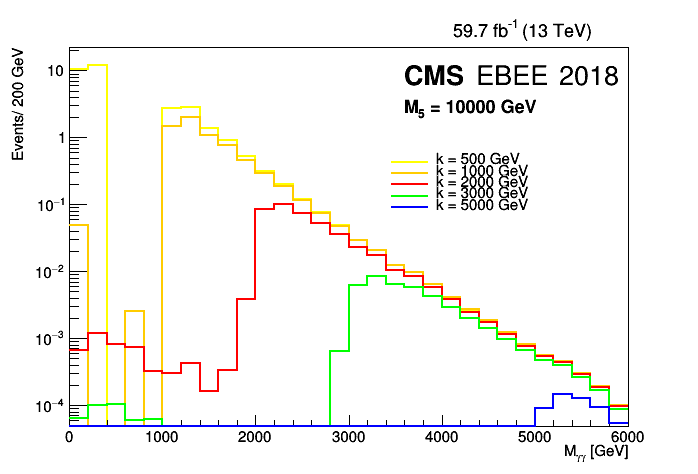
\includegraphics[angle=0,width=0.48\textwidth]{fig/2018EBEE.png}
%     \caption{Signal shapes for the clockwork signal after the final selection for a fixed value of $M_5$ = 10 TeV and varying values of $k$ normalized to the total integrated luminosity for EB-EB events (left) and EB-EE events (right), respectively.}
%     \label{fig:CWSignal}
% \end{figure}


% \begin{figure}[htbp!]
%     \centering
%     \begin{subfigure}[b]{0.48\textwidth}
%         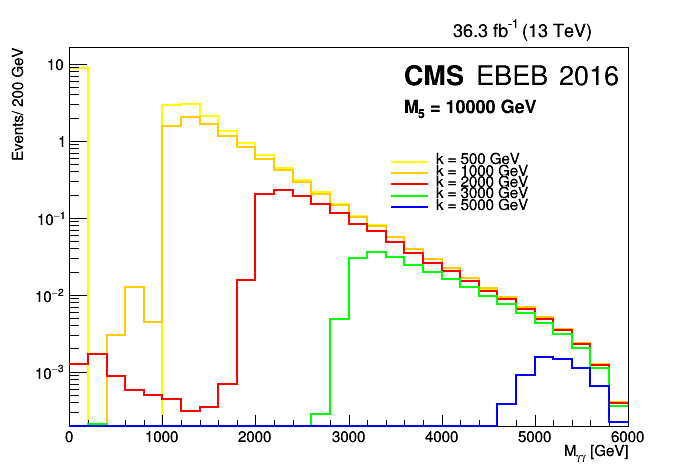
\includegraphics[angle=0,width=\textwidth]{fig/2016EBEB.png}
%         \caption{}
%     \end{subfigure}
%     \hfill
%     \begin{subfigure}[b]{0.48\textwidth}
%         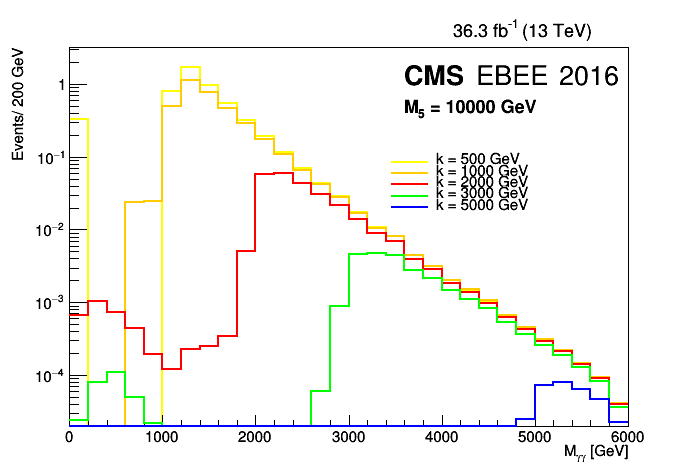
\includegraphics[angle=0,width=\textwidth]{fig/2016EBEE.png}
%         \caption{}
%     \end{subfigure}
%     \vspace{1em}
    
%     \begin{subfigure}[b]{0.48\textwidth}
%         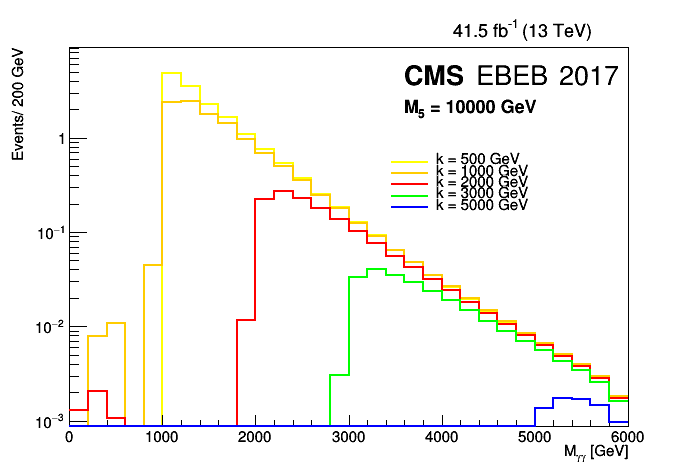
\includegraphics[angle=0,width=\textwidth]{fig/2017EBEB.png}
%         \caption{}
%     \end{subfigure}
%     \hfill
%     \begin{subfigure}[b]{0.48\textwidth}
%         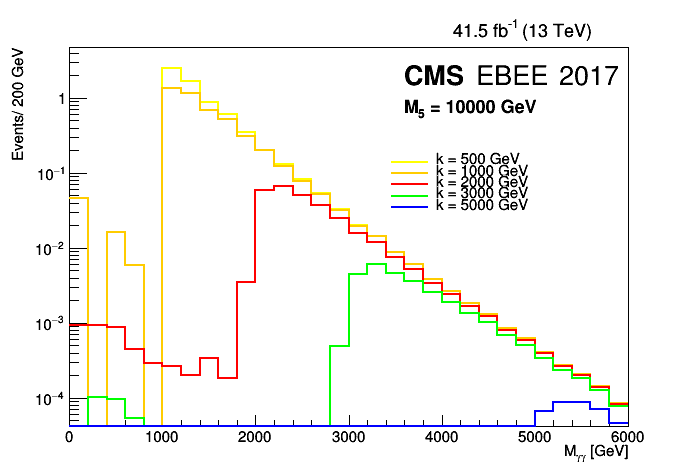
\includegraphics[angle=0,width=\textwidth]{fig/2017EBEE.png}
%         \caption{}
%     \end{subfigure}
%     \vspace{1em}
    
%     \begin{subfigure}[b]{0.48\textwidth}
%         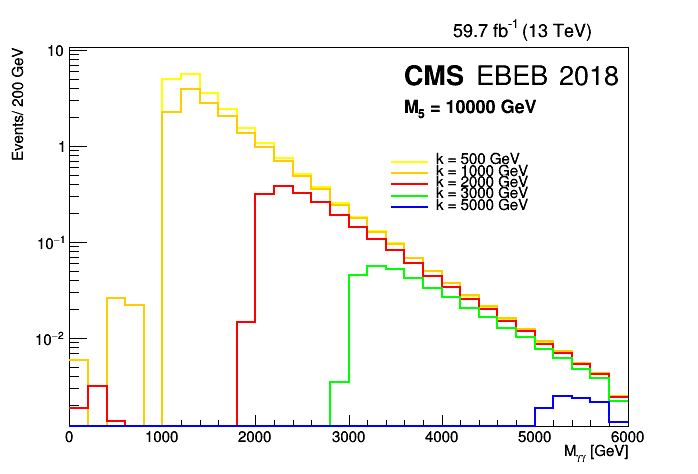
\includegraphics[angle=0,width=\textwidth]{fig/2018EBEB.png}
%         \caption{}
%     \end{subfigure}
%     \hfill
%     \begin{subfigure}[b]{0.48\textwidth}
%         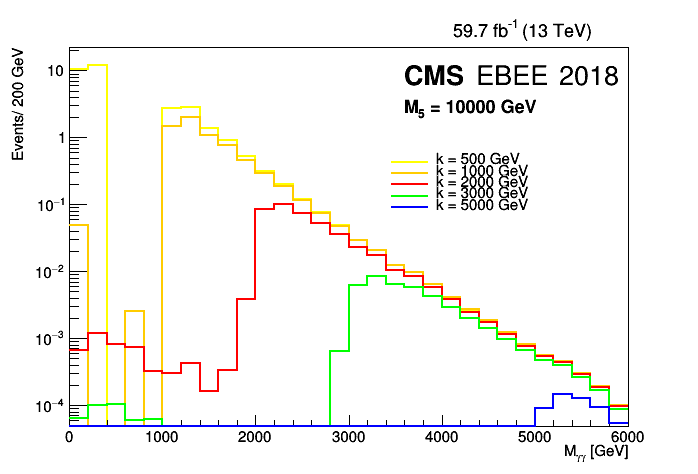
\includegraphics[angle=0,width=\textwidth]{fig/2018EBEE.png}
%         \caption{}
%     \end{subfigure}
%     \caption{Signal shapes for the clockwork signal after the final selection for a fixed value of $M_5$ = 10 TeV and varying values of $k$ normalized to the total integrated luminosity for EB-EB events (left) and EB-EE events (right), respectively.}
%     \label{fig:CWSignal}
% \end{figure}

% \begin{figure}[htbp!]
%     \centering
%     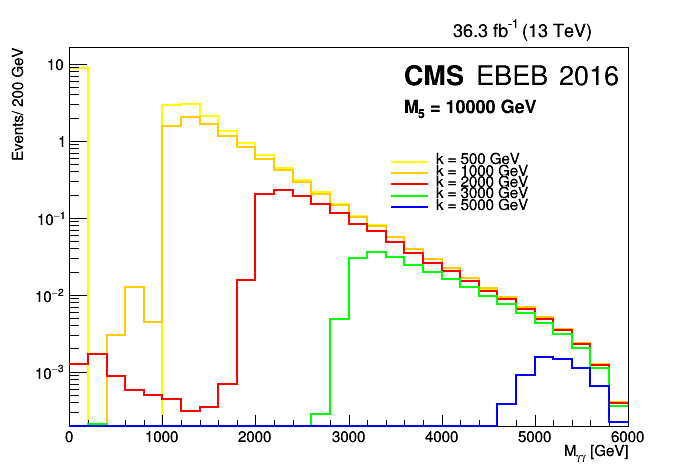
\includegraphics[angle=0,width=0.45\textwidth]{fig/2016EBEB.png}\hspace{0.05\textwidth}
%     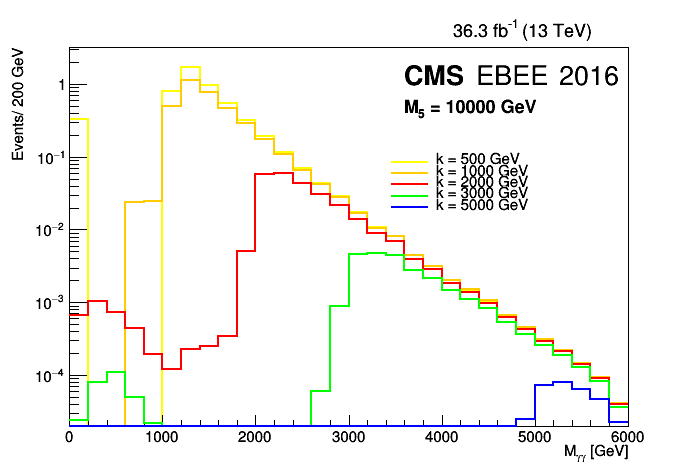
\includegraphics[angle=0,width=0.45\textwidth]{fig/2016EBEE.png}\\[0.5em]
%     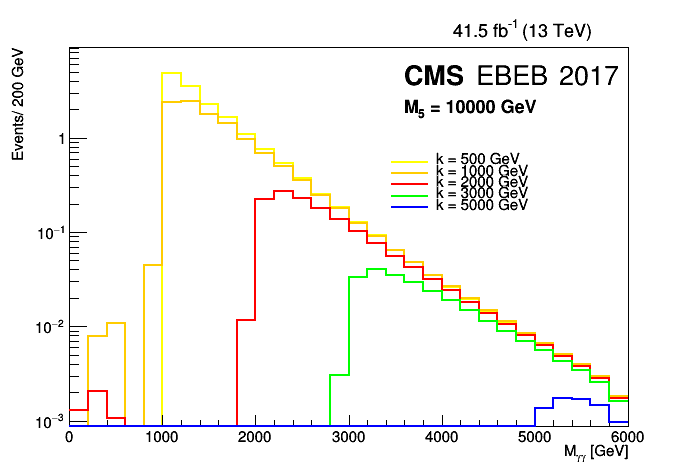
\includegraphics[angle=0,width=0.45\textwidth]{fig/2017EBEB.png}\hspace{0.05\textwidth}
%     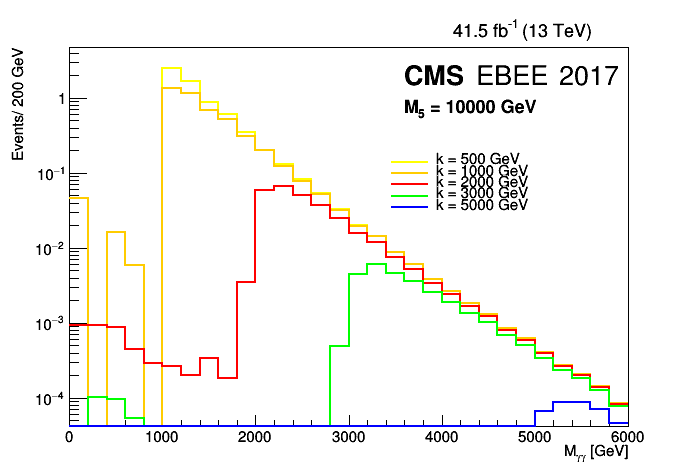
\includegraphics[angle=0,width=0.45\textwidth]{fig/2017EBEE.png}\\[0.5em]
%     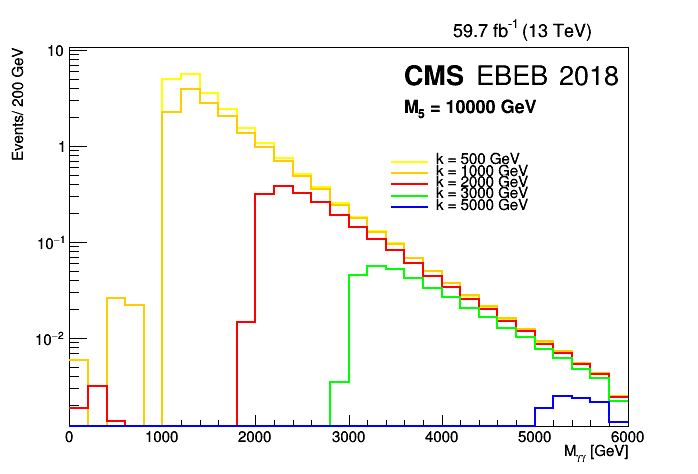
\includegraphics[angle=0,width=0.45\textwidth]{fig/2018EBEB.png}\hspace{0.05\textwidth}
%     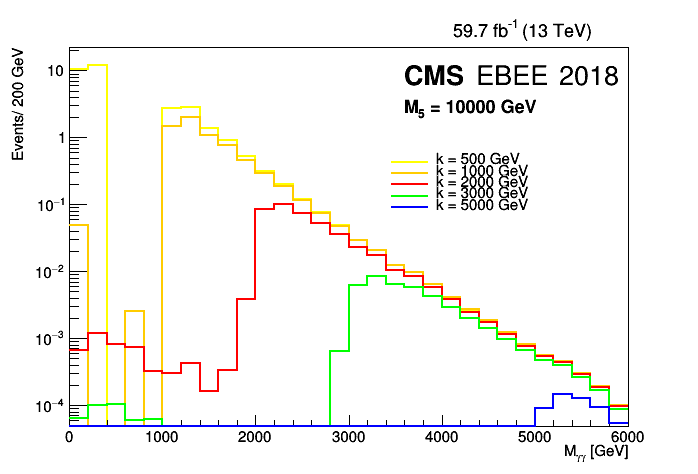
\includegraphics[angle=0,width=0.45\textwidth]{fig/2018EBEE.png}
%     \caption{Signal shapes for the clockwork signal after the final selection for a fixed value of $M_5 = 10~\TeV$ and varying values of $k$ normalized to the total integrated luminosity for EB-EB events (left) and EB-EE events (right), respectively.}
%     \label{fig:CWSignal}
% \end{figure}

% \begin{figure}[htbp!]
%     \centering
%     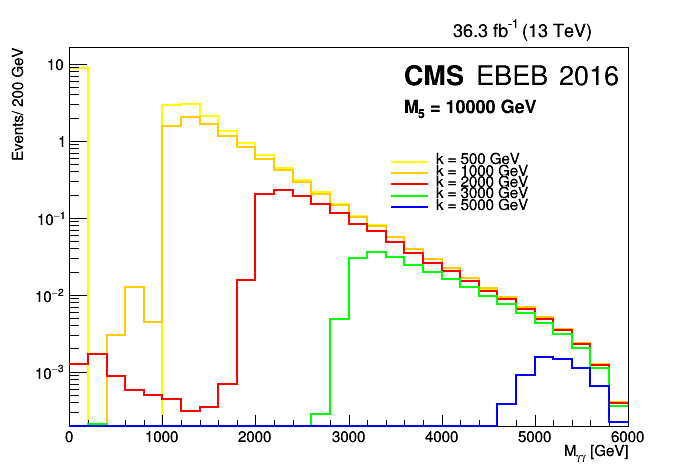
\includegraphics[angle=0,width=0.45\textwidth]{fig/2016EBEB.png}\hspace{0.05\textwidth}
%     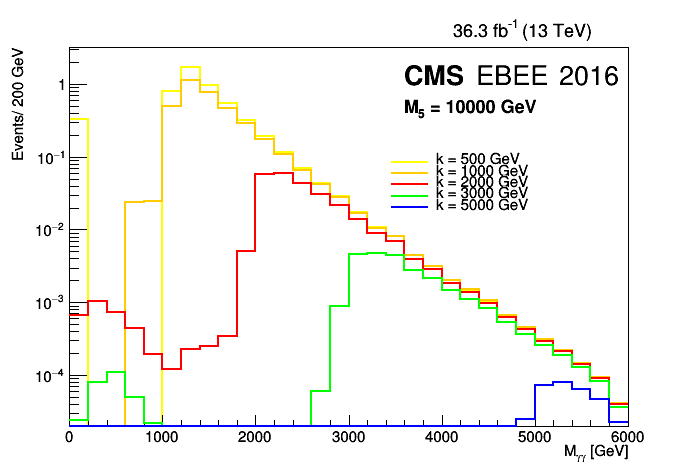
\includegraphics[angle=0,width=0.45\textwidth]{fig/2016EBEE.png}\\[0.5em]
%     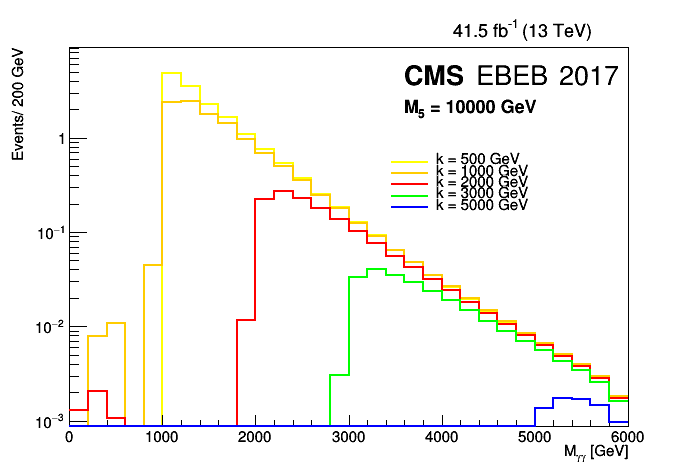
\includegraphics[angle=0,width=0.45\textwidth]{fig/2017EBEB.png}\hspace{0.05\textwidth}
%     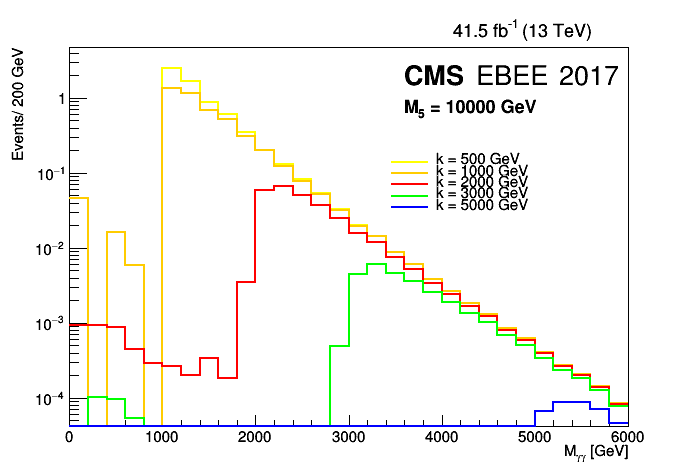
\includegraphics[angle=0,width=0.45\textwidth]{fig/2017EBEE.png}\\[0.5em]
%     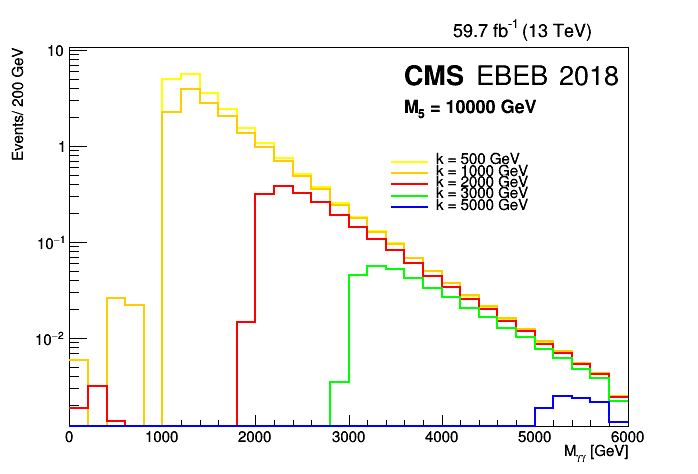
\includegraphics[angle=0,width=0.45\textwidth]{fig/2018EBEB.png}\hspace{0.05\textwidth}
%     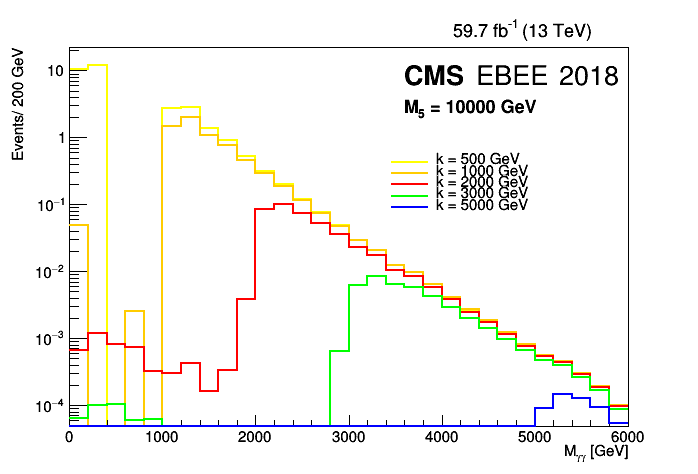
\includegraphics[angle=0,width=0.45\textwidth]{fig/2018EBEE.png}
%     \caption{Signal shapes for the clockwork signal after the final selection for a fixed value of $M_5 = 10~\TeV$ and varying values of $k$ normalized to the total integrated luminosity for EB-EB events (left) and EB-EE events (right), respectively.}
%     \label{fig:CWSignal}
% \end{figure}

% \begin{figure}[htbp!]
%     \centering
%     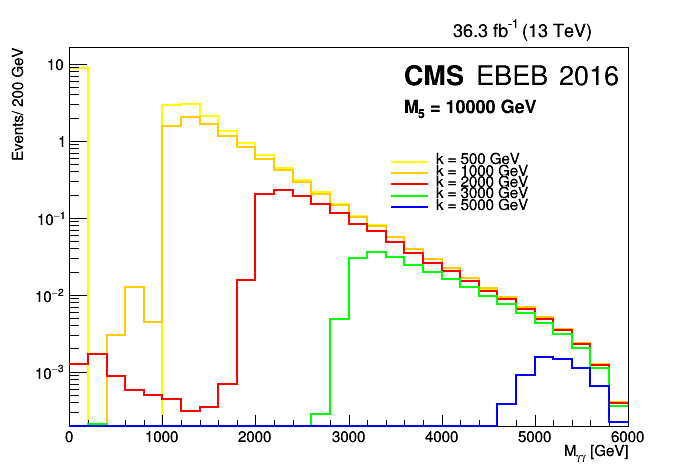
\includegraphics[angle=0,width=0.45\textwidth]{fig/2016EBEB.png}\hfill
%     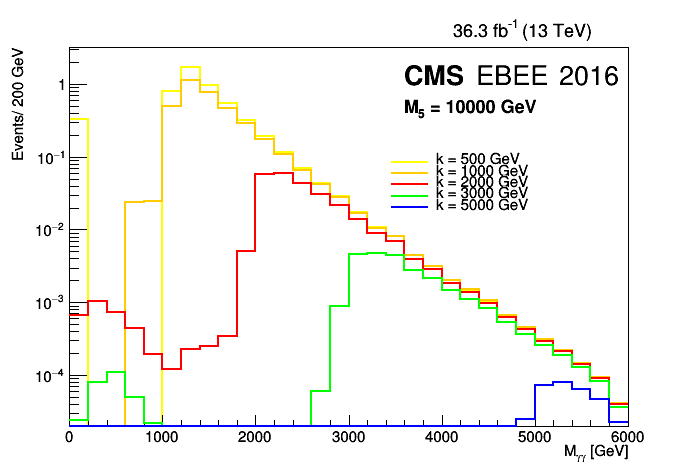
\includegraphics[angle=0,width=0.45\textwidth]{fig/2016EBEE.png}\\[0.5em]
%     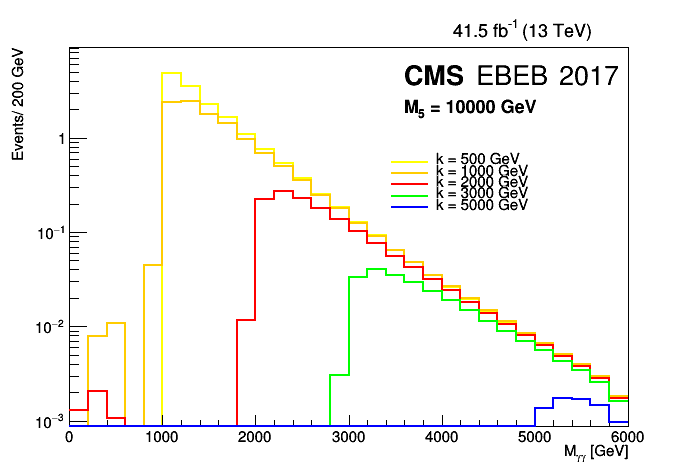
\includegraphics[angle=0,width=0.45\textwidth]{fig/2017EBEB.png}\hfill
%     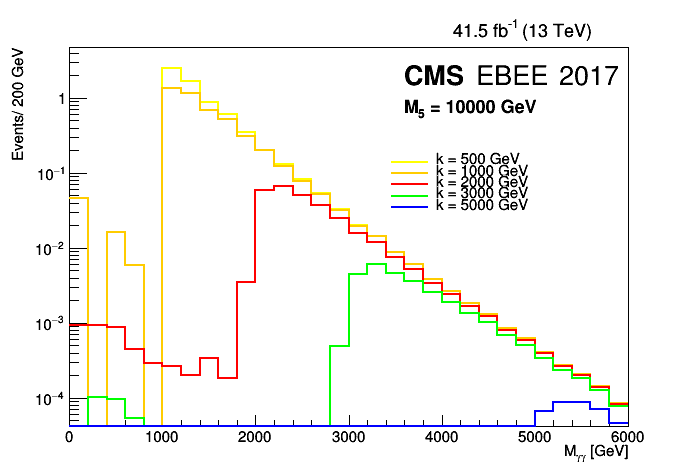
\includegraphics[angle=0,width=0.45\textwidth]{fig/2017EBEE.png}\\[0.5em]
%     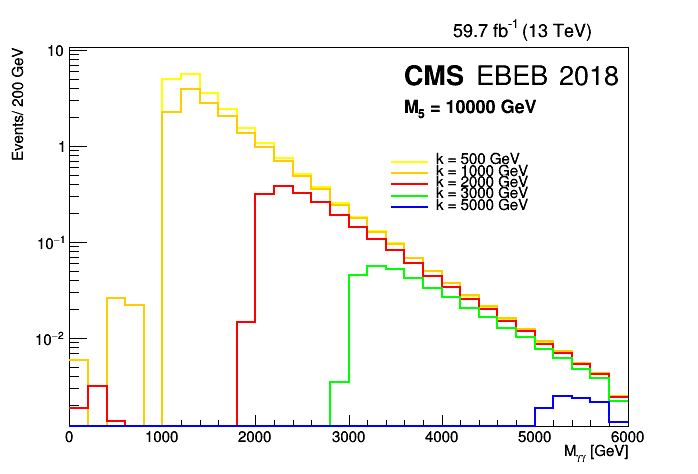
\includegraphics[angle=0,width=0.45\textwidth]{fig/2018EBEB.png}\hfill
%     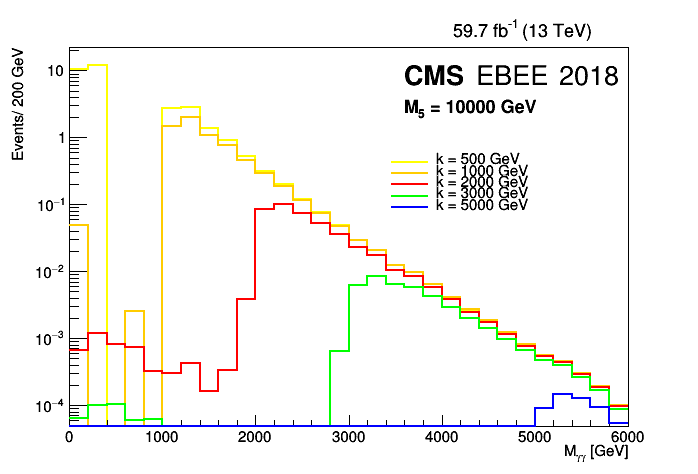
\includegraphics[angle=0,width=0.45\textwidth]{fig/2018EBEE.png}
%     \caption{Signal shapes for the clockwork signal after the final selection for a fixed value of $M_5 = 10~\TeV$ and varying values of $k$ normalized to the total integrated luminosity for EB-EB events (left) and EB-EE events (right), respectively.}
%     \label{fig:CWSignal}
% \end{figure}

\begin{figure}[htbp!]
\caption{Signal shapes for the clockwork signal after the final selection for a fixed value of $M_5 = 10~\TeV$ and varying values of $k$ normalized to the total integrated luminosity for EB-EB events in the left and EB-EE events in the right, respectively.}
\begin{center}
 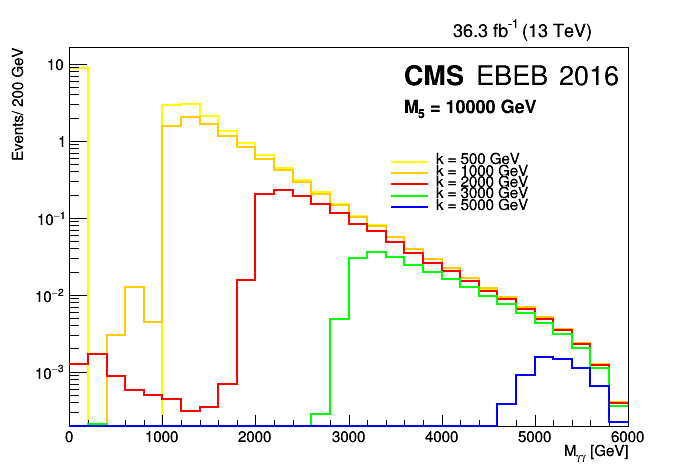
\includegraphics[angle=0,width=0.45\textwidth]{fig/2016EBEB.png}\hfill
    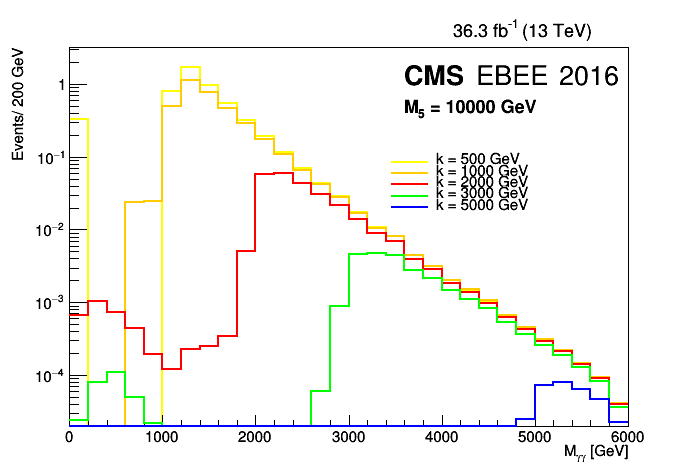
\includegraphics[angle=0,width=0.45\textwidth]{fig/2016EBEE.png}\\[0.5em]
    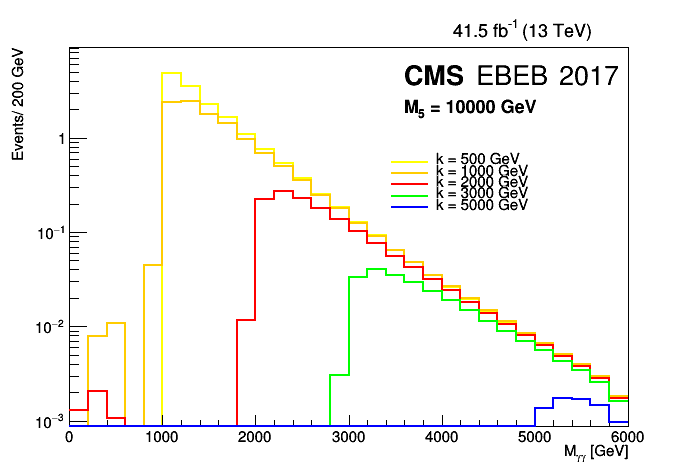
\includegraphics[angle=0,width=0.45\textwidth]{fig/2017EBEB.png}\hfill
    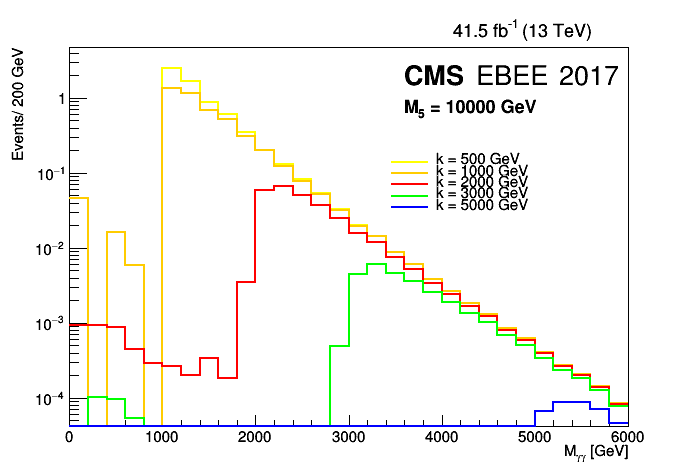
\includegraphics[angle=0,width=0.45\textwidth]{fig/2017EBEE.png}\\[0.5em]
    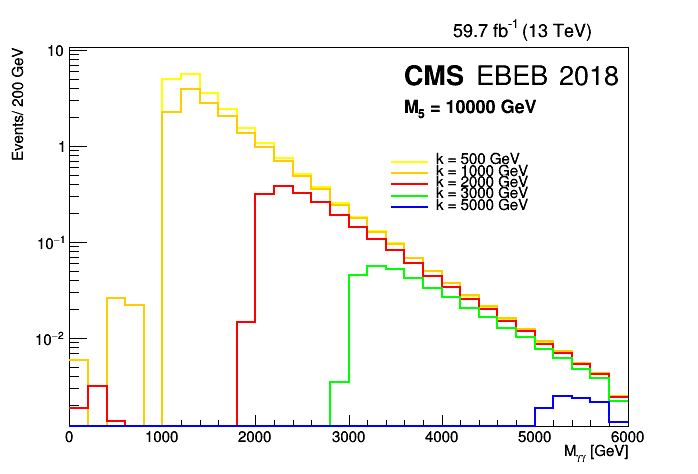
\includegraphics[angle=0,width=0.45\textwidth]{fig/2018EBEB.png}\hfill
    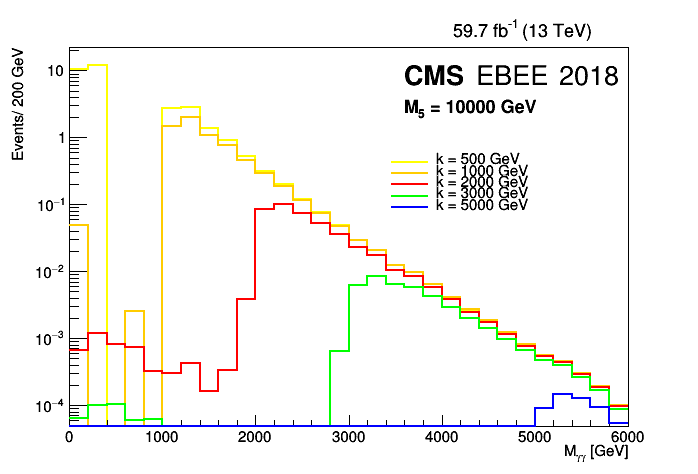
\includegraphics[angle=0,width=0.45\textwidth]{fig/2018EBEE.png}
\end{center}
\label{fig:CWSignal}
\end{figure}


% \begin{figure}[htbp!]
% \centering
% 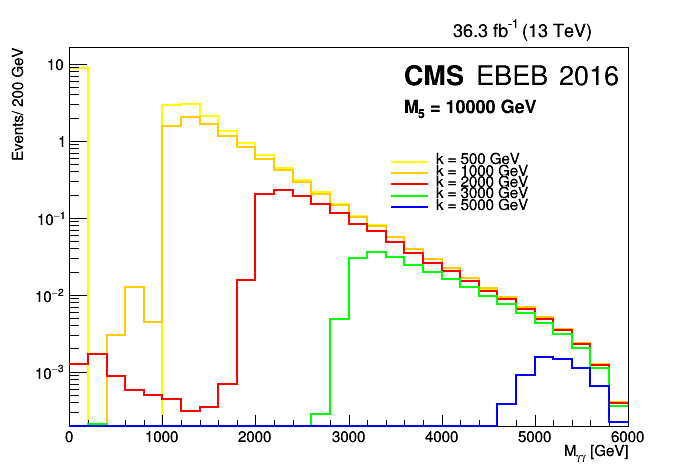
\includegraphics[angle=0,width=0.45\textwidth]{fig/2016EBEB.png}
% 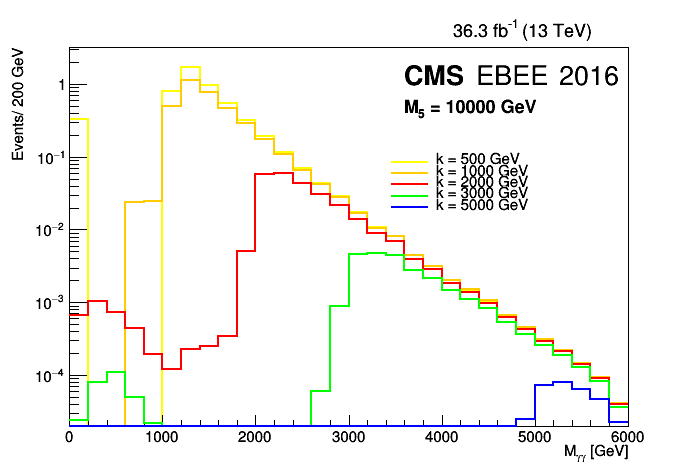
\includegraphics[angle=0,width=0.45\textwidth]{fig/2016EBEE.png}
% 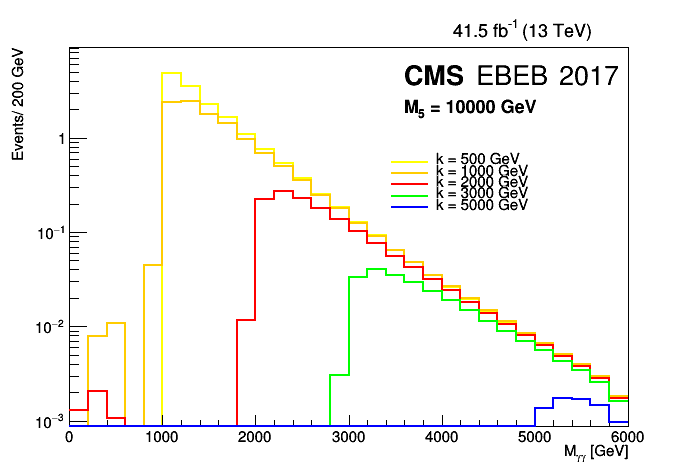
\includegraphics[angle=0,width=0.45\textwidth]{fig/2017EBEB.png}
% 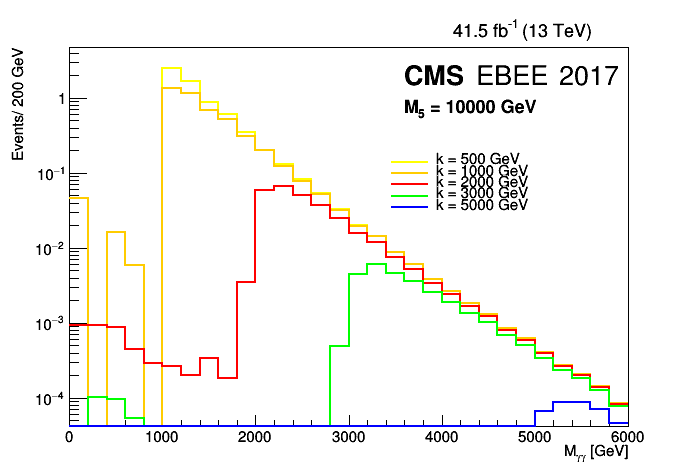
\includegraphics[angle=0,width=0.45\textwidth]{fig/2017EBEE.png}
% 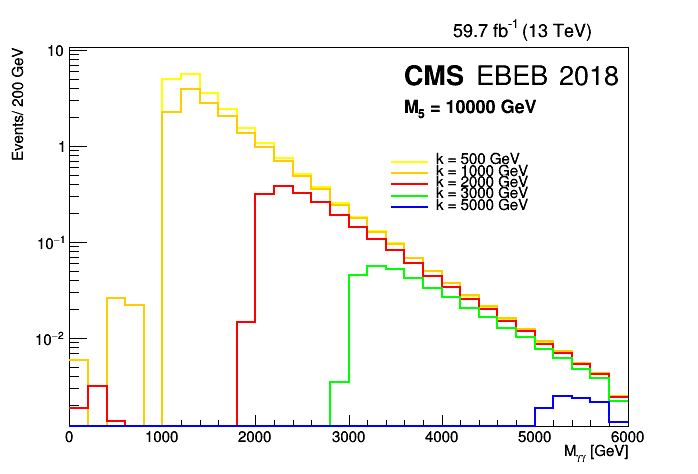
\includegraphics[angle=0,width=0.45\textwidth]{fig/2018EBEB.png}
% 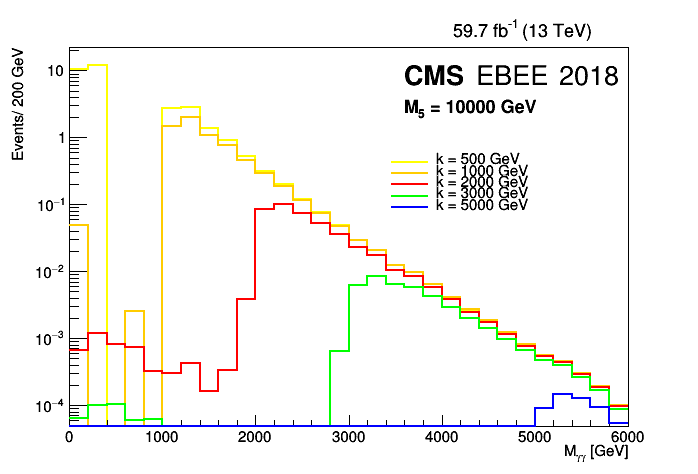
\includegraphics[angle=0,width=0.45\textwidth]{fig/2018EBEE.png}
% \caption{Signal shapes for the clockwork signal after the final selection for a fixed value of $M_5 = 10~\TeV$ and varying values of $k$ normalized to the total integrated luminosity for EB-EB events (left) and EB-EE events (right), respectively.}
% \label{fig:CWSignal}
% \end{figure}

The signal yields for the clockwork model after the final selection and normalized to the total luminosity are shown in Figure~\ref{fig:CWSignal} for EB-EB and EE-EE events. It is immediately noticeable that the shapes differ substantially from those predicted by the ADD model as shown in Figure~\ref{fig:ADDsignal}. When k is small, the distributions are falling as much in the same way that the SM background does, just not as steeply. This provides us with an important experimental challenge in controlling our irreducible background while still providing sufficient discrimination. 

Because the ADD samples are generated together with the SM contribution to account for the interference, the background-subtracted ADD prediction suffers from large statistical uncertainties at low $m_{\gamma\gamma}$. For the ADD model, this is not a problem because the SM contributions completely dominate, but for the clockwork model, this is problematic because the clockwork can predict a large excess even at low values of $m_{\gamma\gamma}$ when $k$ is small. To mitigate this issue, we stitch together positive interference GRW and negative interference Hewett samples with different values of $\Lambda_{T}$. ADD samples with low $\Lambda_{T}$ have larger ADD contributions at low $m_{\gamma\gamma}$ so this helps with the statistics. Even then, we are only able to make statistically reliable predictions for the clockwork signals for $m_{\gamma\gamma} > 900$ GeV with the samples we have. Higher $\Lambda_{T}$ samples are used at higher $m_{\gamma\gamma}$ to deal with the unitarity truncation when $\sqrt{\hat{s}} > \Lambda_{T}$. 

% \begin{figure}[tbp!]
% \begin{center}
% 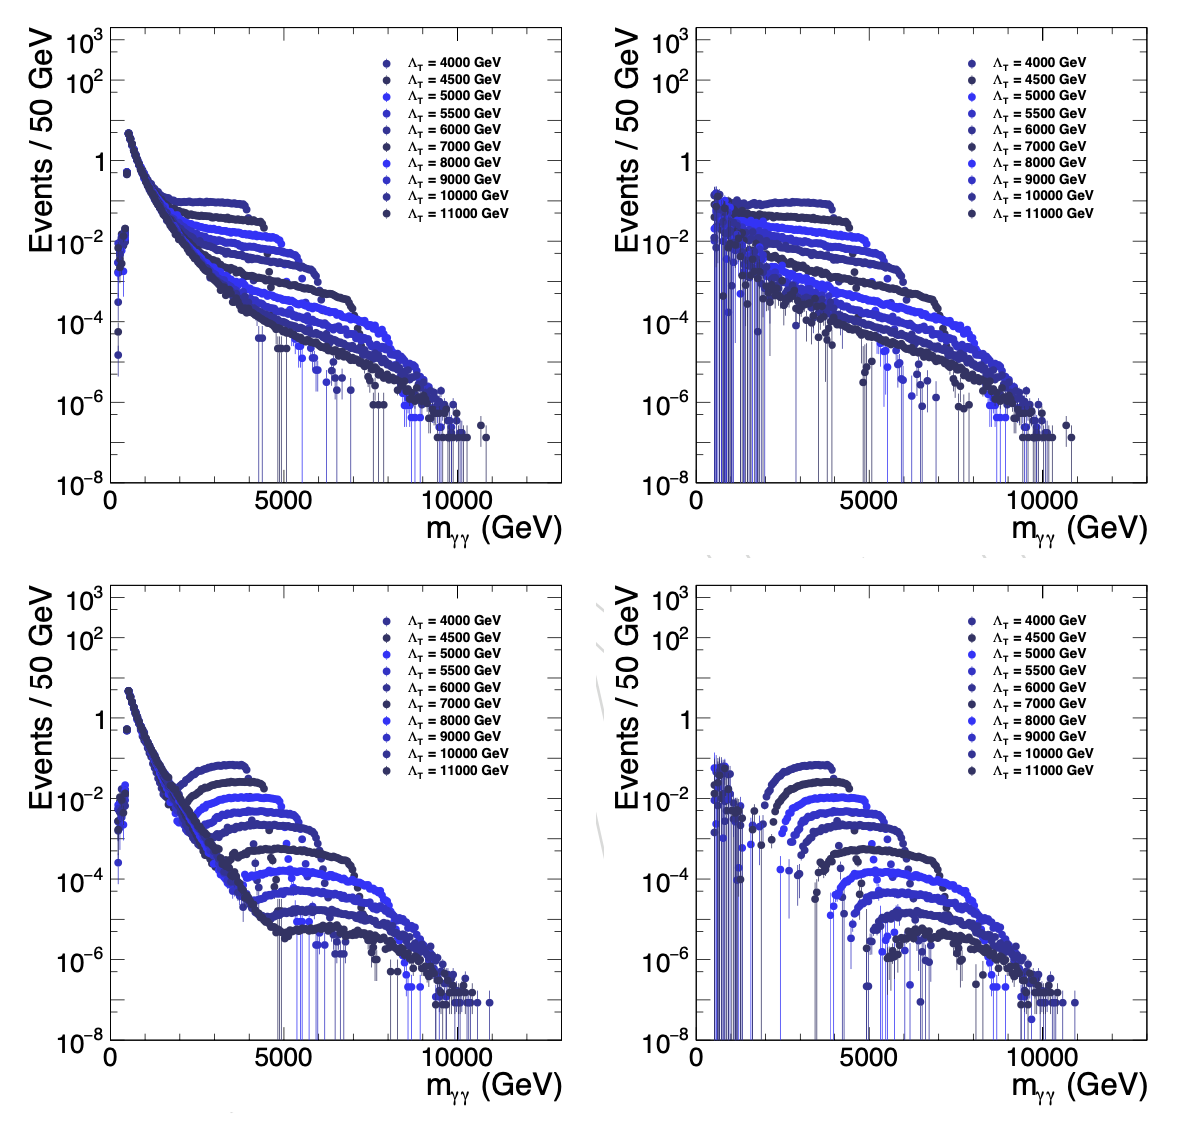
\includegraphics[angle=0,width=0.9\textwidth]{fig/ADD2017Shapes.png}
% \end{center}
% \caption{The $m_{\gamma\gamma}$ distribution in signal events for the generated values of $\Lambda_T$ before (left) and after (right) subtraction of SM background. The upper (lower) plots show signals generated assuming positive (negative) interference with the SM background. The plots were generated using the 2017 ADD samples and are normalized to an integrated luminosity of 1\fbinv.}
% \label{fig:ADDSignal.png}
% \end{figure}


\subsection{Unparticles to Diphoton}
In this dissertation we also show our preliminary studies on both the spin-0 (scalar) and spin-2 (tensor) Unparticles to diphoton production. As shown in Figure~\ref{fig:UnparticlesFeynmanDiagram}, the Unparticles can be produced through $q\Bar{q}$ annihilation and gg fusion subprocess with spin-0 and spin-2 unparticles appearing as propagators. 

% \footnote{The propagator is the probability amplitude for a particle to travel with a certain energy and momentum, in time.}. 

\begin{figure}[!htbp]
	\caption{Leading-order Feynman diagrams for the Unparticles to two photons.}
	\centering
    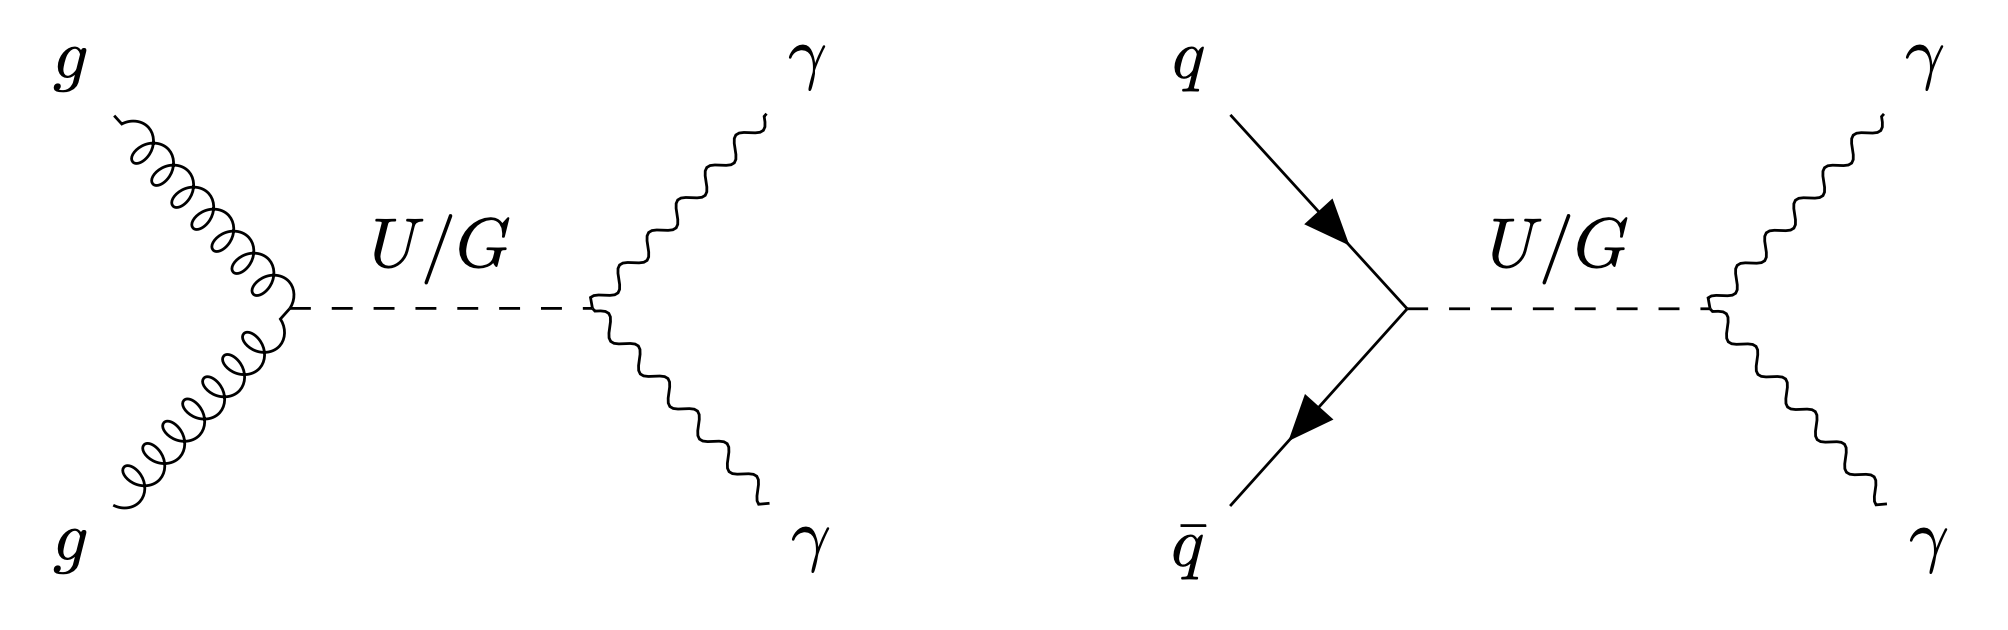
\includegraphics[scale=0.4]{fig/Unparticles_Graviton.png}
	\label{fig:UnparticlesFeynmanDiagram}
\end{figure}

Our search space is a two-dimensional parameter space, where $d_u$ is the scale dimension parameter and $\Lambda_{U}$, is the Unparticle renormalization scale. To simplify our search, we set the strength of the Unparticle Coupling to the Standard Model $\lambda = 1$. 

The Unparticles model produce diphoton events via virtual graviton exchange and appear as a non-resonant excess in the diphoton invariant mass spectrum similar to the ADD model \cite{Ask:2009pv}. The Unparticles signal samples listed in Table~\ref{table:UnparticlesSamples} were produced at leading order (LO) using \PYTHIA~8.2~\cite{Sjostrand:2008za},
with the \texttt{NNPDF}3.1 LO set of parton distribution functions as found in the event tune, \texttt{TuneCP2}~\cite{Sirunyan:2019dfx}.

For our first look, we span the 2-dimensional parameter space as follows: for each spin we chose $du$ values $1.1$, $1.5$, $1.9$. For numerical reasons\cite{KumarEtal:2008}, it is recommended that $du$ be restricted from $1.01$ to $1.9$ as values beyond this search space cannot be probed due to some coefficients in the interference and matrix-element rapidly varying. The choices for $\Lambda_U$ vary for each $du$. For spin-0, the $\Lambda_U$ choices for each $du$ are as follows: $du$ = $1.1$, $\Lambda_U$ = $4000, 8000, 10000$ GeV, $du$ = $1.5$ and $1.9$, $\Lambda_U$ = $2000, 2500, 3500$ GeV. For spin-2, $du$ = $1.1$, $1.5$, $\Lambda_U$ = $2000, 2500, 3000$ GeV, and $1.9$, $\Lambda_U$ = $2000, 2500, 3500$ GeV, with the mass ranges $M$ $500-1000$, $1000-2000$, $2000-\infty$ for $\Lambda_U$ less than $3000$ GeV. For $\Lambda_U > 3000$ GeV, the mass bins are $500-1000$, $1000-2000$, $2000-3000$ and $3000-\infty$ in units of GeV.

\begin{figure}[!htbp]
	\caption{The 2D-plane with the parameters of the Unparticles model.
The 95\% CL upper limits on signal strength (y-axis) vs the $\Lambda_U$ (x-axis) and the lower limits on $\Lambda_U$ for the unparticles model.
On the left spin 0, on right spin 2. Top to bottom, $d_{u}$ parameter value: 1.1, 1.5 and 1.9 (Credits to Antonios Agapitos).}
	\centering
% 	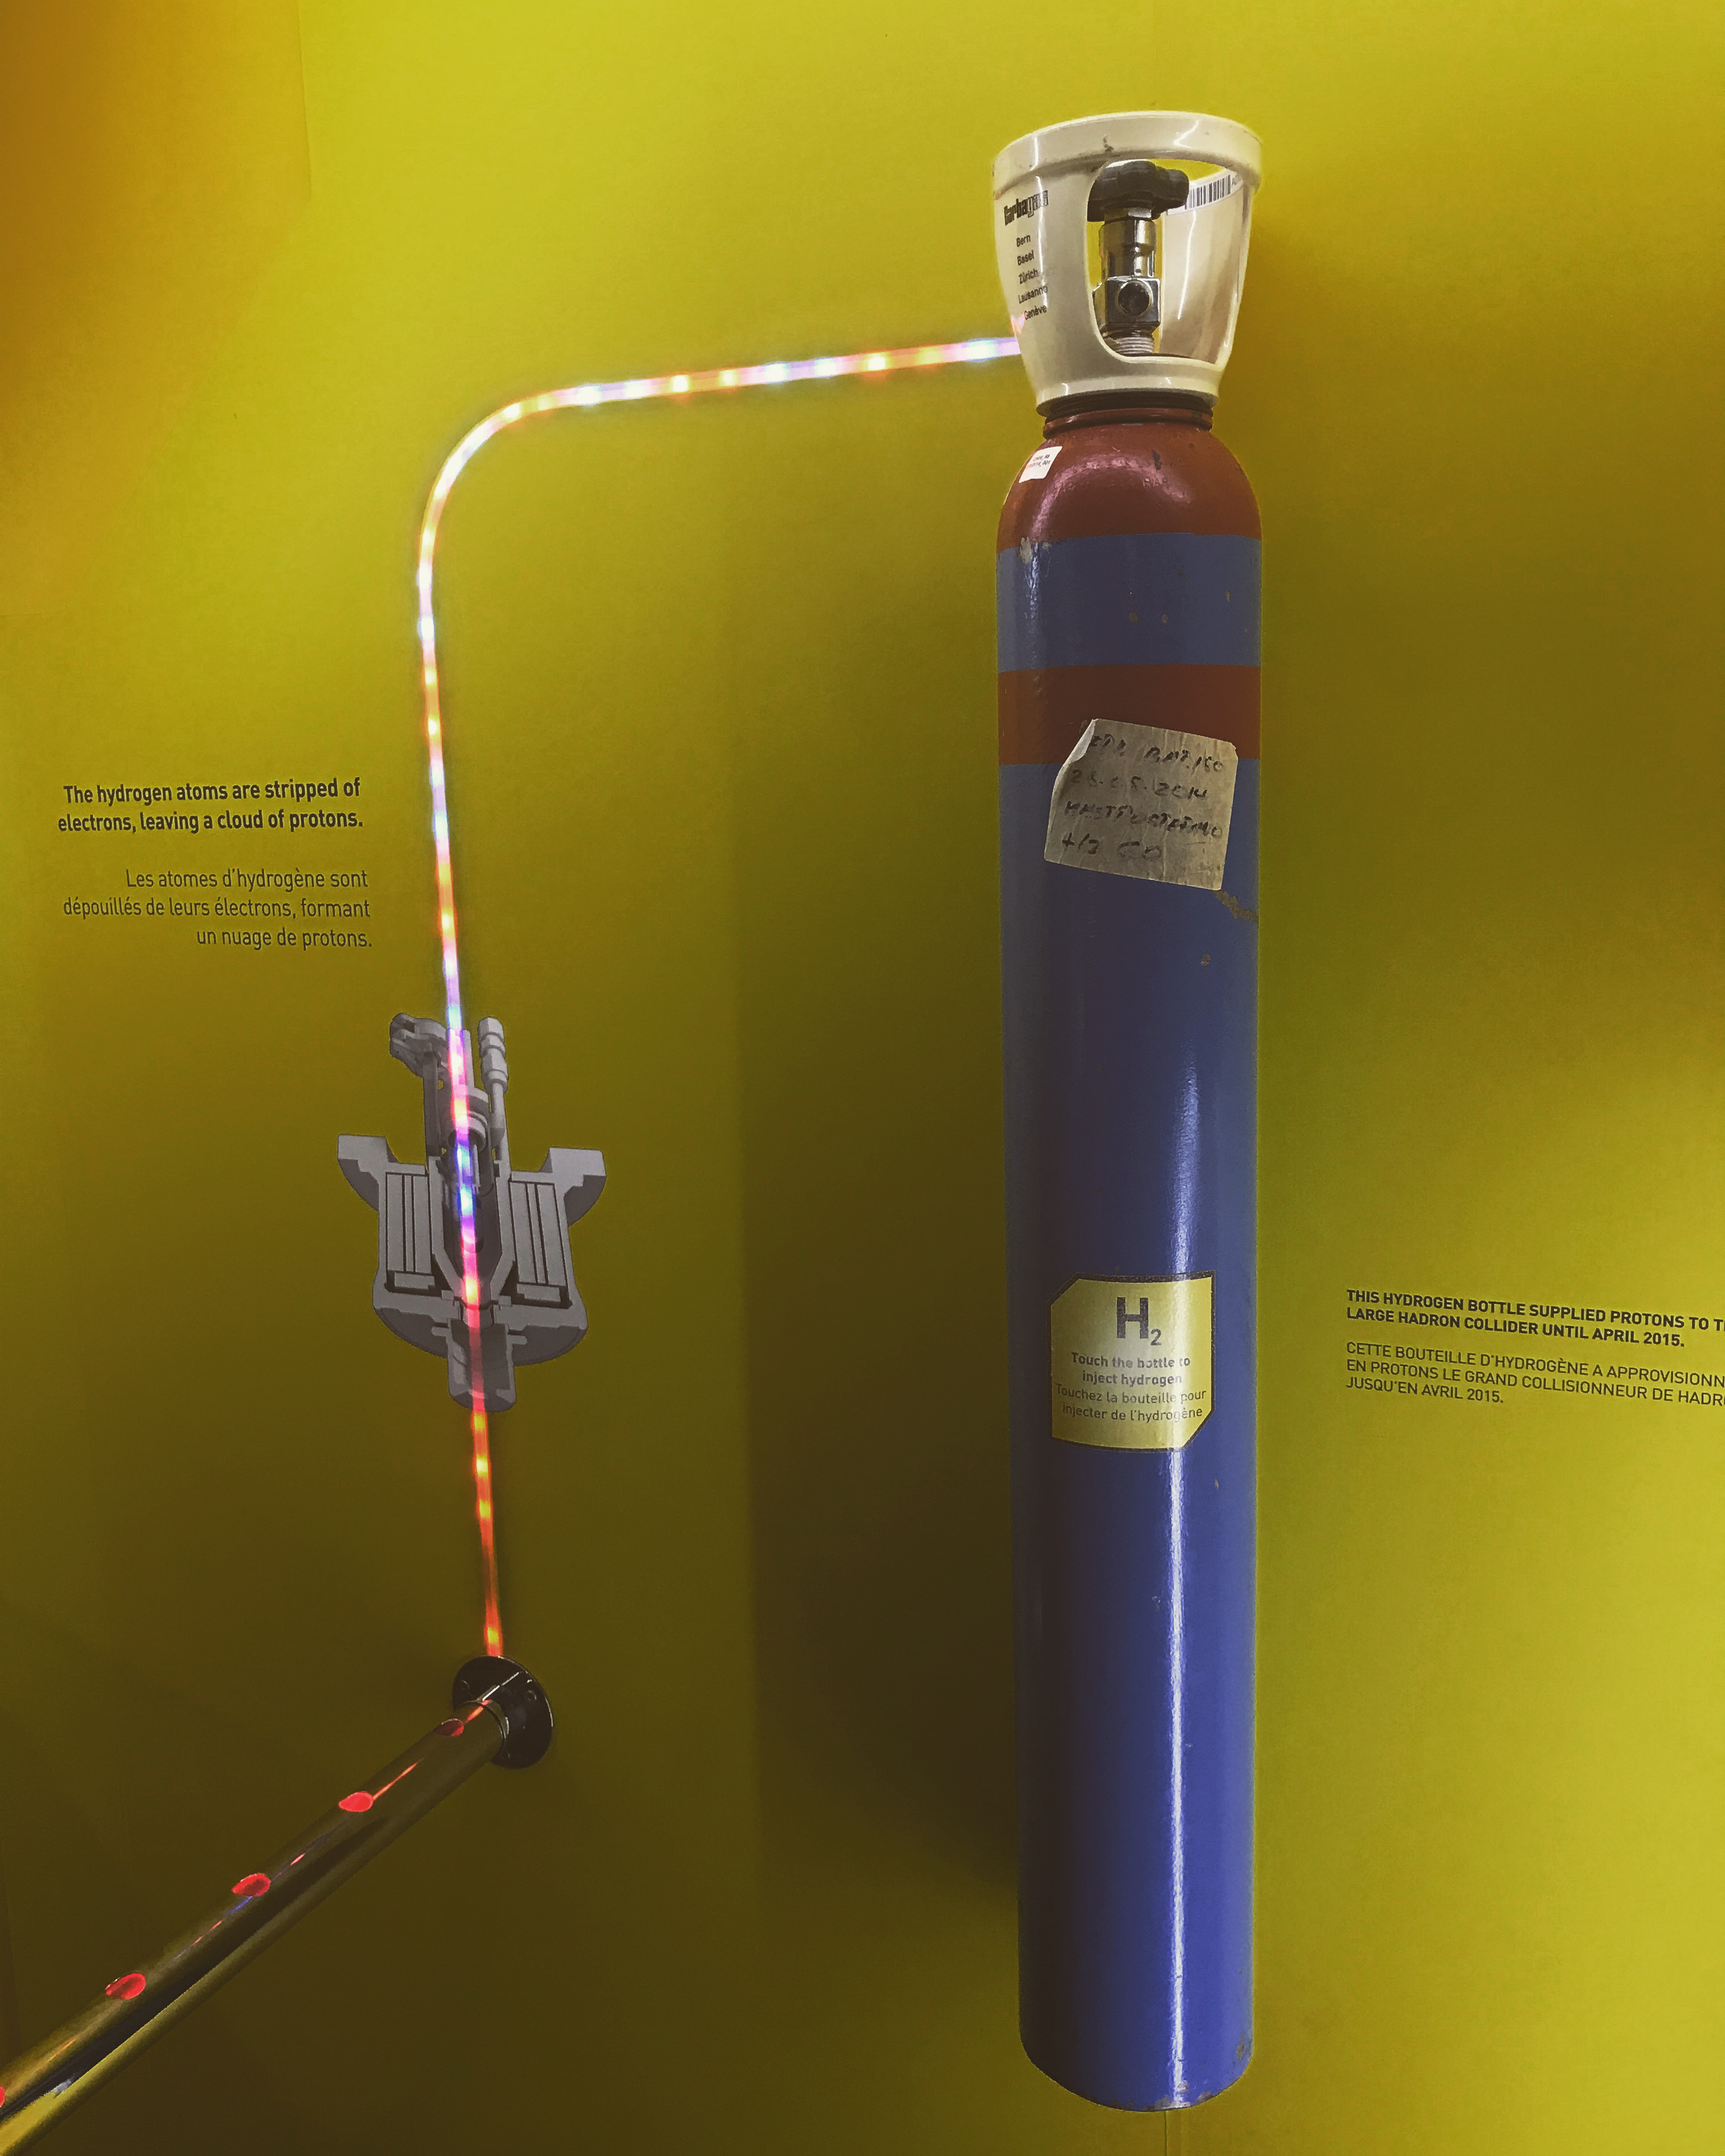
\includegraphics[scale=0.038]{fig/H2Bottle.JPG}
    \includegraphics[scale=0.3]{fig/Unpar_plane.png}
	\label{fig:UnparticlesSearchSpace}
\end{figure}

% \subsection{Pythia8 Monte Carlo Event Generator}

We used \PYTHIA8.3~\cite{Sjostrand:2008za} to generate the events with Unparticles decaying into two photons (see Appendix~\ref{ch:appendix_sample_cards} for a sample \PYTHIA card.).

The \mgg distributions for the signal samples are displayed in Figure~\ref{fig:UnparSignal} both before and after the subtraction of the SM background. 


\begin{figure}[htbp!]
\caption{The $m_{\gamma\gamma}$ distribution in unparticle signal events for the generated values of $\Lambda_U$. The upper (lower) plots show signals generated assuming spin-0 (spin-2) $du=1.9$. The left (right) plots show before (after) SM background subtraction. These plots were generated using the 2018 Unparticles samples.}
\begin{center}
\includegraphics[angle=0,width=0.48\textwidth]{fig/UnparToGG_Spin0_du1p9_TuneCP2_13TeV_pythia8_2018.pdf}
\includegraphics[angle=0,width=0.48\textwidth]{fig/UnparToGG_Spin0_du1p9_TuneCP2_13TeV_pythia8_2018_bkg_sub.pdf}
\includegraphics[angle=0,width=0.48\textwidth]{fig/UnparToGG_Spin2_du1p9_TuneCP2_13TeV_pythia8_2018.pdf}
\includegraphics[angle=0,width=0.48\textwidth]{fig/UnparToGG_Spin2_du1p9_TuneCP2_13TeV_pythia8_2018_bkg_sub.pdf}
\end{center}
\label{fig:BkgSub}
\end{figure}


 % \PYTHIA8 is used for the leading-only (LO) prediction that will be later used for background subtraction for the signal samples. The Born and Box diagrams are treated separately in the event-generator. 

\newpage
% \section{References}
% \renewcommand{\bibsection}{}%removes the spaces and unwanted references heading from the list
% \begin{singlespacing}
% \bibliographystyle{apsrev}
% \bibliography{Ref_SignalSimClockwork.bib}
% \end{singlespacing}\par